%
% A sample LaTeX thesis file using ppfcmthesis class.
%
% This file is UNOFFICIAL and NOT (URRENTLY) ENDORSED by the University.
%
% Written by Dawid Weiss.
%
% Class options:
%     pl        Polish headers and typesetting.
%     en        English headers and typesetting.
%
\documentclass[polish,a4paper,oneside]{../fcm-unofficial/ppfcmthesis}

\usepackage[utf8]{inputenc}
\usepackage[OT4]{fontenc}
\usepackage{url}
\usepackage{../fcm-utils/fcmcode}

% Put your thesis details here
\author{Mirosław Begier}
%\title{JDBMeasure -- benchmark do testowania wydajności systemów zarządzania bazami danych}
\title{Benchmark systemu zarządzania bazą danych}
\ppsupervisor{dr~hab.~inż.~Maciej Drozdowski,~prof.PP}
\ppyear{2006}

\begin{document}
% 

% title page, front matter, contents list.
\maketitle\cleardoublepage%
\thispagestyle{empty}\vspace*{\fill}\noindent\begin{center}%
Tutaj karta pracy dyplomowej;\\w oryginale w wersji do archiwum PP, w kopiach ksero.\end{center}\vfill\cleardoublepage%
\thispagestyle{empty}\vspace*{\fill}\vfill\noindent
\hspace{2cm}Chciałbym w tym miejscu złożyć najserdeczniejsze podziękowania mojemu promotorowi, dr~hab.~inż.~Maciejowi~Drozdowskiemu, 
dzięki któremu powstała ta praca, za jego życzliwość, zaangażowanie, cenne uwagi oraz czas poświęcony na przeprowadzone konsultacje.
\\
\begin{flushright}
Mirosław Begier
\end{flushright}
\cleardoublepage%
\frontmatter\pagenumbering{roman}{\small\tableofcontents}\cleardoublepage%

% main body of your thesis starts here.
\mainmatter%

\chapter{Wstęp}

Rozdział ten ma przybliżyć czytelnikowi motywacje jak i zakres realizowanej pracy magisterskiej, 
zawiera również krótki opis planu realizacji prac.

\section{Motywacje}\label{sect:Motywacje}

Obecnie na rynku dostępnych jest kilka benchmarków do testowania wydajności DBMS~\cite{DBMS}, 
różnią się one pomiędzy sobą zarówno zakresem testowanych właściwości, systemami dla których
są przeznaczone np.: OLTP (\english{Online Transaction Processing}~\cite{OLTP}) 
czy OLAP (\english{On Line Analytical Processing}~\cite{OLAP}),
jak i obsługiwanymi DBMS. Posiadają jednak z reguły pewne istotne ograniczenia:
\begin{itemize}
\item związane są z jednym niemodyfikowalnym modelem bazy danych i obciążenia,
\item występują często jako specyfikacja -- tj. wymagają implementacji specyfikacji benchmarku niezależnie dla każdego DBMS,
\item umożliwiają testowanie jednego konkretnego DBMS.
\end{itemize}
Czy jednak istnieje możliwość, stworzenia benchmarku na tyle uniwersalnego,
by możliwe było definiowanie dla niego różnych modeli nie tylko baz danych,
ale również modeli obciążenia? Ponadto by modele te, zapisane w sposób niezależny
od konkretnego DBMS, mogły być wykorzystywane przez benchmark do testowania różnych DBMS?
Czy możliwe jest stworzenie benchmarku nie tylko przeznaczonego do porównywania wydajności
różnych DBMS, ale również do szukania najlepszego modelu bazy danych dla tworzonego rozwiązania, systemu?
Odpowiedzią na powyższe pytania ma być niniejszy benchmark i związana z nim praca magisterska.

\section{Cel i zakres pracy}

Celem pracy jest stworzenie oprogramowania (benchmarku) do testowania wydajności
\definicja{systemów zarządzania bazą danych} (\akronim{DBMS}, \english{Database Management System}). 
Benchmark powinien symulować rzeczywisty model bazy danych np.: sklep internetowy, bank, lub hurtownię itp.
Model obciążenia powinien się skalować, tzn. umożliwiać zwiększanie rozmiaru w miarę wzrostu prędkości komputera.
Należy przeprowadzić testy prędkości dla operacji języka \definicja{SQL} (\english{Structured Query Language}~\cite{SQL}) typu select, insert, update, delete.
Testy powinny obejmować zależności prędkości od rozmiarów bazy danych i od liczby klientów (jednocześnie podłączonych). 
Wyniki trzeba wszechstronnie opracować w postaci tekstowej i graficznej (średnie, mody, mediany, histogramy).
Językiem programowania będzie Java, do łączenia z bazami danych użyty zostanie interfejs \definicja{JDBC} (\english{Java Database Connectivity}~\cite{JDBC1}).

Praca nad projektem została podzielona wstępnie na kilka etapów. Poniżej zamieszczono, krótki ich opis.
\subsection{Zapoznanie się z istniejącymi rozwiązaniami}

Tworzenie oprogramowania do testowania wydajności różnego typu elementów systemów komputerowych,
w tym systemów zarządzania bazami danych, nie jest zagadnieniem nowym, dlatego przed rozpoczęciem prac, 
należy zapoznać się z istniejącymi rozwiązaniami, by ,,nie odkrywać Ameryki na nowo''.
W tym celu przewidziano zapoznanie się z produktami organizacji \definicja{TPC} (\english{Transaction Processing Performance Council}) -- \url{http://www.tpc.org } ,
a w szczególności ze specyfikacją benchmarku TPC-C dostępną pod adresem \url{http://www.tpc.org/tpcc}.

\subsection{Stworzenie modelu rozwiązania}

W tym etapie głównym celem będzie stworzenie modelu benchmarku, tak by model ten
spełniał zarówno cele pracy, jak i był odpowiedzią na pytania postawione w podrozdziale \ref{sect:Motywacje}.

\subsection{Implementacja benchmarku na niskim poziomie}

W pierwszej kolejności zostanie stworzona struktura benchmarku tj.: struktura komunikacyjna
dla zapewnienia wymiany danych pomiędzy serwerem, a klientami RTE (\english{Remote Terminal Emulator}).
Wytworzone zostaną także elementy związane z generacją populacji bazy danych, analizą modeli, przygotowywaniem skryptów testowych,
oraz ich wykonywaniem na RTE.

\subsection{Testowanie struktury różnych DBMS}

Struktura testu zostanie przetestowana na kilku DBMS min.: Oracle 10g~\cite{Oracle1}, PostgresSQL 8.1~\cite{PostgreSql1}, MySQL 5.0~\cite{MySql1}.

\subsection{GUI serwera}

W tym kroku zostanie stworzone GUI(\english{Graphical User Interface}~\cite{GUI}) dla serwera benchmarku,
dla klientów RTE -- interfejs pozostanie tekstowy. Interfejs ten będzie umożliwiał
tworzenie modeli przy pomocy formularzy, zarządzanie klientami RTE, oraz
przeprowadzanie procedury testu. 

\subsection{Generator raportów}

Ostatnim etapem prac będzie dodanie do systemu generatora raportów, w postaci tekstowej
i graficznej. Dodane zostaną histogramy obrazujące rozkład czasów odpowiedzi dla
operacji i transakcji.

\chapter{Benchmarki baz danych}\label{chap:teo}

Niniejszy rozdział omawia wybrane elementy pomiaru wydajności baz danych. Został tutaj 
omówiony między innymi jeden z typowych benchmarków OLTP--TPC-C, a także różnice pomiędzy nim, 
a tworzonym rozwiązaniem.

\section{TPC}

\akronim{TPC} (\english{Transaction Processing Performance Council}, \url{www.tpc.org} ) jest 
organizacją zajmującą się badaniem wydajności przetwarzania transakcyjnego.
\begin{figure}[t]
\begin{center}
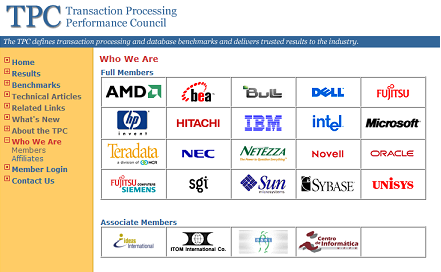
\includegraphics[width=0.8\linewidth]{figures/tpc/tpc_members.png}
\end{center}
\caption{Członkowie TPC~\cite{TPC1}}\label{rys:tpc_members}
\end{figure}
Organizacja ta przygotowuje specyfikacje testów służących do badania i porównywania wydajności m.~in.: 
systemów zarządzania bazami danych (\akronim{SZBD}, \english{DBMS}). Na podstawie tych specyfikacji tworzone są benchmarki, 
czyli narzędzia pomiaru wydajności, dla konkretnych DBMS. Z uzyskanych wyników publikowane są raporty 
umożliwiające porównanie wydajności różnych rozwiązań. Organizacja TPC skupia ekspertów z zakresu baz danych, reprezentujących
duże, znane przedsiębiorstwa (zob.~rys.~\ref{rys:tpc_members}). Niestety członkostwo nie jest darmowe~\cite{TPC1}:

\begin{quote}
Full Members of the TPC participate in all aspects of the TPC's work, including
development of benchmark standards and setting strategic direction. 
Full Membership costs $\$15\,000$ per calendar year.
\end{quote}

\noindent%
W związku z powyższym w grupie tej brakuje przedstawicieli rozwiązań niekomercyjnych jak
MySQL czy PostgreSQL.

Specyfikacje testów TPC różnią się między sobą zakresem badanych właściwości. 
Zakres ten dla konkretnej specyfikacji odpowiada właściwością konkretnego typu DBMS.
Poniżej wymieniono benchmarki TPC dotyczące baz danych.

\begin{description}
\item[TPC-A (OLTP) (1989)] 
TPC-A jest odmianą benchmarku debetowo-kredytowego OLTP (1985). Model bazy danych reprezentuje
w nim bank. Baza danych składa się z czterech typów rekordów: rachunek, kasjer, oddział, historia.
Miarą efektywności jest wydajność mierzona liczbą transakcji na jedną sekundę. 90\% transakcji powinno mieć czas
odpowiedzi 2 sekundy lub krótszy. Benchmark ten jest przestarzały. 

\item[TPC-B (\english{database stress test}) (sierpień 1990)]
W tym benchmarku nie ma użytkowników, linii komunikacyjnych czy terminali. Jest to test obciążeniowy,
dotyczący głównie operacji dyskowych. Benchmark ten nie jest testem OLTP i podobnie jak TPC-A jest przestarzały.

\item[TPC-C (OLTP) (lipiec 1992)]
Benchmark ten jest testem OLTP, bardziej złożonym od TPC-A. Występuje w nim mieszanka 5 różnych typów transakcji,
z których mierzy się czasy dla jednej, a pozostałe pełnia rolę szumu. Model bazy danych jest typową hurtownią składającą 
się z 9 relacji o określonej, skalowalnej liczbie rekordów i powiązań. Miarą efektywności jest tutaj liczba wykonanych 
transakcji typu ,,nowe zamówienie'' na minutę. Bliższe informacje odnośnie tego benchmarku znajdują się w dalszej części rozdziału.  

\item[TPC-D (kwiecień 1995)]
TPC-D reprezentuje szeroki zakres aplikacji wspomagania decyzji, które wymagają złożonych długotrwających zapytań,
na dużych skomplikowanych strukturach danych~\cite{TPC1}.

\item[TPC-H]
Benchmark ten jest kolejnym testem przeznaczonym dla systemów bazodanowych zorientowanych na wspomaganie decyzji,
w których występują duże, złożone struktury danych i duże, złożone zapytania. W przeciwieństwie do TPC-D, w benchmarku
tym podczas tego typu operacji wykonywane są równolegle pewne operacje modyfikujące dane.

\item[TPC-R] 
TPC-R jest benchmarkiem podobnym do TPC-H, lecz dodatkowo uwzględnia możliwość optymalizacji zapytań na podstawie
zaawansowanej wiedzy odnośnie zapytań.

\item[TPC-W]
Jest to benchmark transakcji dla aplikacji opartych o interfejs stron WWW. Test ten porusza wiele
cech charakterystycznych w tego typu systemach takich jak:
\begin{itemize}
    \item występowanie wielu sesji użytkowników,
    \item dynamiczne generowanie stron z jednoczesnym dostępem do bazy danych i jej uaktualnianiem,
    \item komunikacja w oparciu o protokół HTTP.
\end{itemize}
Miarą efektywności jest tutaj liczba interakcji ze stroną na sekundę. Wielokrotne interakcje ze stroną WWW
są wykorzystywane w celu symulacji rzeczywistej sprzedaży detalicznej. Każda interakcja jest przedmiotem
indywidualnych ograniczeń czasowych.

\item[TPC-App (\english{Application Server and Web Services Benchmark})]
TPC-App jest benchmarkiem serwerów aplikacji i technologii WebServices. Benchmark ten wykorzystuje w testach
komunikację opartą o dokumenty XML i protokół SOAP. Uwzględnia również wielosesyjność systemów oraz
dynamiczną konstrukcję odpowiedzi WebServices opartą o dostęp i modyfikację bazy danych. Baza danych składa się z
wielu tabel złożonych z dużej liczby kolumn, wierszy i powiązań. Od systemu wymaga się spełnienia właściwości 
\akronim{ACID}, zapewniających integralność transakcji. Miarą wydajności jest tutaj liczba obsłużonych
żądań.
\end{description}

Z powyższej listy specyfikacji wynika jeden istotny wniosek -- nie istnieje 
jeden uniwersalny benchmark umożliwiający badanie wydajności całej gamy istniejących
systemów zarządzania bazami danych. Również budowane rozwiązanie jest ukierunkowane
na badanie cech SZBD głównie typu OLTP. Dlatego też w kolejnym rozdziale zostanie
przybliżona specyfikacja benchmarku TPC-C.

\section{Benchmark TPC-C}

Benchmark TPC-C jest specyfikacją modelu pomiarowego dla systemów zarządzania bazami danych. 
Model ten opisuje strukturę bazy danych zgodnej z OLTP, jak i metodologię dokonywania pomiarów.
Specyfikacja ta jest niezależna od konkretnego DBMS. TPC-C nie jest zatem narzędziem pomiaru wydajności,
jest raczej specyfikacją budowy i użytkowania takiego narzędzia dla konkretnego DBMS. Specyfikacja 
ta rozwijana jest od połowy 1992 roku przez organizację TPC (aktualna wersja specyfikacji to wersja 5.6).

Warto też w tym miejscu wymienić cechy charakterystyczne OLTP, są to:
\begin{itemize}
\item proste operacje SQL typu select, insert, update oraz delete,
\item duża liczba klientów i wielodostęp,
\item najważniejszym parametrem jest średni czas wykonania komendy sql,
\item współbieżność transakcji, rozwiązywanie konfliktów,
\item miliony transakcji.
\end{itemize}
A zatem pomiary dokonywane przez benchmarki OLTP wymagać będą tych cech.

Specyfikacja TPC-C zawiera opis bazy danych, dla której dokonywane mają być testy. Struktura
bazy nie może ulegać odstępstwom, w zależności od konkretnej implementacji benchmarku.
Opis ten zawiera zarówno omówienie relacji, powiązań między nimi, jak i populację bazy danych
przed rozpoczęciem testów (zob.~rys.~\ref{rys:tpc_db_structure} oraz rys.~\vref{rys:tpc_db_structure2}). 
W ramach populacji omówiona jest nie tylko liczba rekordów w poszczególnych relacjach 
w zależności od parametru skalującego, lecz również rozkład wartości 
poszczególnych atrybutów i ich cechy szczególne takie jak unikalność, możliwość
przyjmowania wartości pustych.

\begin{figure}[p]
\begin{center}
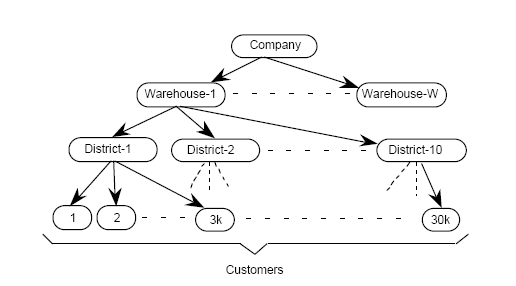
\includegraphics[width=\linewidth]{figures/tpc/tpc_db_structure.png}
\end{center}
\caption{Struktura bazy danych dla TPC-C~\cite{TPC1}}\label{rys:tpc_db_structure}
\end{figure}

\begin{figure}[p]
\begin{center}
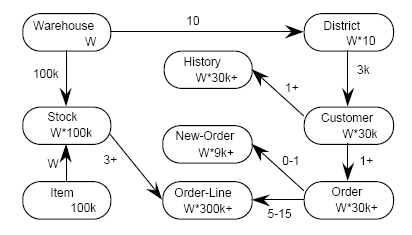
\includegraphics[width=\linewidth]{figures/tpc/tpc_db_structure2.png}
\end{center}
\caption{Struktura bazy danych dla TPC-C~\cite{TPC1}}\label{rys:tpc_db_structure2}
\end{figure}
\afterpage{\clearpage} % wymuś stronę rysunków po tej stronie.

TPC-C specyfikuje pięć typowych transakcji dla zaproponowanego modelu bazy danych.
To właśnie te transakcje, o określonej proprocji występowania, poddawane są testom. 
Warto zauważyć, że dla dowolnego schematu relacji zbiór wszystkich możliwych transakcji jest olbrzymi,
nie chodzi zatem o to by przetestować wszystkie te transakcje, lecz aby wybrać
do przetestowania najbardziej typowe -- te, z którymi mielibyśmy do czynienia
w bazie użytkowej. Ważnym elementem są scenariusze, które określają prawdopodobieństwo
wykonania operacji danego typu, po zakończeniu operacji innego typu. Omówione zostały również 
kwestie skalowalności populacji.

Dla każdej z 5 transakcji omówiono sposób generowania danych wejściowych,
profil jak i szczegółowe informacje dotyczące wymagań odnośnie wejścia/wyjścia 
terminali pomiarowych -- \akronim{RTE} (\english{Remote Terminal Emulator)}.

Rozdział 3 specyfikacji omawia właściwości jakie powinien spełniać system
podczas przeprowadzania pomiarów~\cite{TPC2}:

\begin{quote}
The ACID (Atomicity, Consistency, Isolation, and Durability) properties of 
transaction processing systems must be supported by the system under test 
during the running of this benchmark.
\end{quote}

Przyjrzymy się bliżej tym właściwościom:
\begin{itemize}
\item atomowość -- system poddawany testom musi gwarantować atomowość transakcji;
\item spójność -- wykonanie transakcji musi powodować przejście bazy danych z jednego stanu spójnego do innego;
\item izolacja -- poziom izolacji transakcji określany jest na podstawie występowania, bądź nie, 4 anomalii,
są nimi: ,,brudny zapis''(\english{Dirty Write}), ,,brudny odczyt''(\english{Dirty Read}), 
,,niepowtarzalny odczyt''(\english{Non-repeatable Read}) oraz ,,fantom''(\english{Phantom}). 
Sposób wyznaczenia poziomu izolacji w zależności od anomalii obrazuje tab.~\vref{tab:isol_tab}.
Dla każdej z 5 transakcji określono poziom izolacji, jaki musi zapewniać system poddawany testom;

\begin{table}[t]
\caption{Poziomy izolacji i anomalie.}\label{tab:isol_tab}
\scriptsize\centering%
\begin{tabular}{c c c c c}
\toprule
Poziom izolacji & \multicolumn{4}{c}{Anomalia} \\ \cmidrule{2-5}
                & Brudny zapis & Brudny odczyt & Niepowtarzalny odczyt & Fantom \\ \midrule
0 & Niemożliwy & Możliwy    & Możliwy   & Możliwy    \\
1 & Niemożliwy & Niemożliwy & Możliwy   & Możliwy    \\
2 & Niemożliwy & Niemożliwy & Niemożliwy& Możliwy    \\
3 & Niemożliwy & Niemożliwy & Niemożliwy& Niemożliwy \\
\bottomrule
\end{tabular}
\end{table}

\item trwałość -- testowany system musi zapewniać trwałość, oznacza to, że w przypadku wystąpienia
awarii, system musi umożliwiać odzyskanie ostatniego stanu spójnego bazy danych sprzed awarii.
\end{itemize}

Specyfikacja TPC-C opisuje również bardzo szczegółowo tworzenie wymaganych raportów.
Zestaw takich metryk po zakończeniu pomiarów powinien być przekazany wraz z wynikami do organizacji TPC-C.
Na rys.~\vref{rys:tpc_required_reporting1} przedstawiono przykładowy raport obrazujący
liczbę transakcji danego typu, w zależności od czasu ich odpowiedzi. Raport ten musi, między innymi, posiadać 
20 równej długości przedziałów na osi $X$, a także oś ta musi mieć długość równą 
4 krotnej długości przypadającej na 90\% transakcji. 

\begin{figure}[p]
\begin{center}
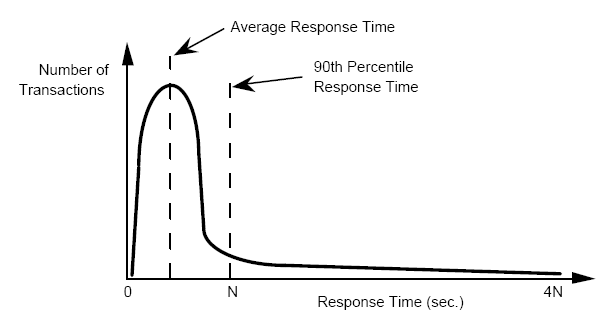
\includegraphics[width=\linewidth]{figures/tpc/tpc_required_reporting1.png}
\end{center}
\caption{Czas odpowiedzi (źródło:~\cite{TPC2}).}\label{rys:tpc_required_reporting1}
\end{figure}

\begin{figure}[p]
\begin{center}
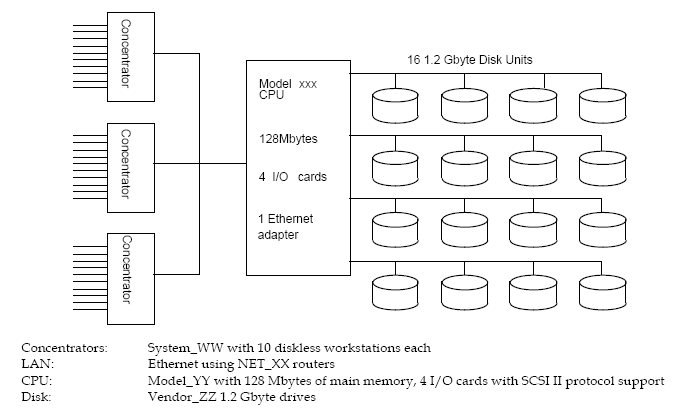
\includegraphics[width=\linewidth]{figures/tpc/tpc_full_disclosure1.png}
\end{center}
\caption{Przykładowy diagram połączeń\cite{TPC2}}\label{rys:tpc_full_disclosure1}
\end{figure}

Nierozerwalną częścią raportu z przeprowadzonych testów są również:
\begin{itemize}
\item Dokładny i szczegółowy opis środowiska, w którym przeprowadzono testy -- opis ten powinien uwzględniać szereg aspektów: 
parametry sprzętu komputerowego, jego liczba, sposób łączenia, sposób konfiguracji SZBD, parametry sieci, opis
systemu operacyjnego i niezbędnego oprogramowania. W tym celu można załączać wszelkiego rodzaju diagramy takie jak
np.~rys.~\vref{rys:tpc_full_disclosure1}.\afterpage{\clearpage}
\item Wycena systemu, w którym przeprowadzono testy -- w skład tej wyceny powinny wejść takie elementy jak sprzęt komputerowy, 
infrastruktura sieciowa, w tym urządzenia sieciowe, system operacyjny jak i inne niezbędne oprogramowanie, SZBD, 
zakup niezbędnych licencji itd. O dużej wadze przywiązywanej przez twórców do tego elementu
świadczyć może poświęcenie wycenie odrębnego rozdziału w specyfikacji.
\end{itemize}

Aby wyniki testów były ważne, tj.~uznane przez TPC, niezbędne jest również przejście pozytywnie
przez procedurę audytu przeprowadzaną przez niezależnych audytorów licencjonowanych
przez organizację TPC. Specyfikacja benchmarku TPC-C zawiera zatem listę kontrolną
na podstawie której przeprowadzany jest audyt, a także dokładny opis tej procedury.

Dopiero po spełnieniu tych wszystkich wymagań wyniki testu TPC-C mogą być opublikowane przez organizację TPC.
Wyniki takie służą do porównywania wydajności poszczególnych SZBD. Na rys.~\vref{rys:tpc_sample_results} 
przedstawiono przykładowe wyniki publikowane przez organizacje TPC. Jest to skrócona wersja wyników. 
Najważniejszymi wskaźnikami są tutaj \akronim{tpmC} (\english{transactions per minute}) 
-- liczba transakcji typu ,,nowe zamówienie'' wykonanych na minutę oraz \akronim{price/tpmC} czyli 
koszt podzielony przez liczbę tych transakcji na minutę.

\begin{figure}[htp]
\begin{center}
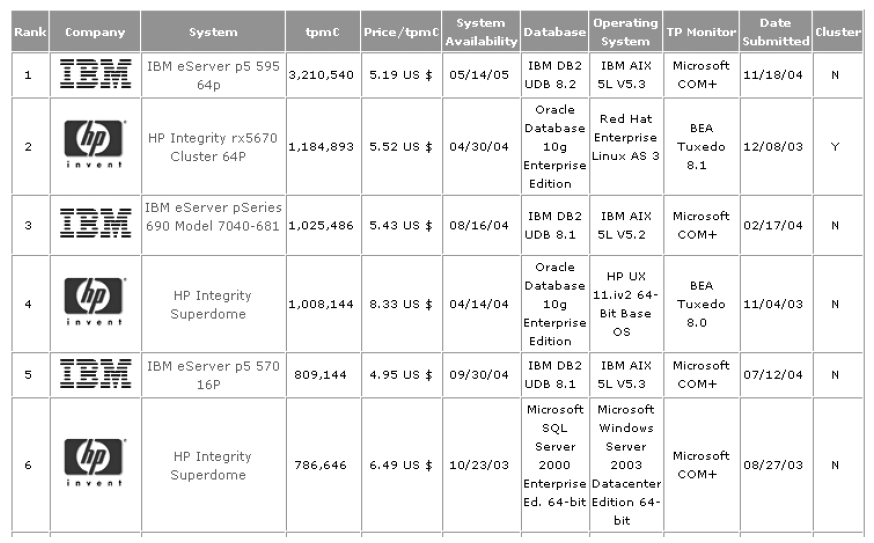
\includegraphics[width=\linewidth]{figures/tpc/tpc_sample_results.png}
\end{center}
\caption{Przykładowe wyniki TPC (źródło: \cite{TPC1}).}\label{rys:tpc_sample_results}
\end{figure}

W związku z tym, iż benchmark ten jest z reguły wykorzystywany przez twórców bazy danych,
gotowych ponieść duże nakłady finansowe, aby uzyskać w teście możliwie jak najlepsze rezultaty,
z punktu widzenia użytkownika najistotniejszym kryterium wydaje się być stosunek ceny zbudowanego systemu,
poddawanego testom, do liczby transakcji obsługiwanych przez ten system w jednostce czasu. 

\section{Podsumowanie}

Z powyższego opisu benchmarku TPC-C można wysnuć kilka istotnych wniosków:

\begin{itemize}
    \item TPC-C jest specyfikacją -- aby przeprowadzić testy wybranego SZBD należy zaimplementować 
    tą specyfikację dla niego.
    \item Niezmienną rzeczą w teście jest ustalony model bazy danych. W przypadku próby sprawdzenia,
    jak na konkretnym SZBD zachowuje się pod względem wydajności, inny model bazy danych, nie można
    posłużyć się tym benchmarkiem.
    \item Benchmark jest przeznaczony do opracowania raportów publikowanych przez TPC. Raporty te służą
    do porównywania nie tylko SZBD, ale całych platform bazodanowych.
\end{itemize}

W przeciwieństwie do powyższych cech, budowany w tej pracy benchmark ma charakteryzować się:
\begin{itemize}
    \item możliwością stworzenia własnych modeli bazy danych i obciążenia bazy danych,
    \item dostępnością predefiniowanych modeli baz danych,
    \item możliwością przeprowadzenia testów na więcej niż jednym SZBD (Oracle, PostgreSQL, MySQL),
    \item uniezależnieniem modelu bazy danych i obciążenia od konkretnego SZBD. 
\end{itemize}

W przeciwieństwie do TPC-C system testujący przygotowany w pracy ma spełniać głównie funkcje użytkowe, 
ze względu na swoją prostotę, ale i elastyczność ma być narzędziem, dostępnym dla zwykłego użytkownika.


\chapter{JDBMeasure - pierwsze spojrzenie}\label{rodz:over}
Rozdział ten zawiera ogólny opis struktury benchmarku, a w szczególności omawia ideę
definicji testu poprzez tworzenie trzech modeli: bazy danych, obciążenia i testu.
Została tutaj także opisana infrastruktura benchmarku tj. podział na aplikacje
serwera i RTE.
\section{Infrastruktura}
Benchmark oparty jest o architekturę klient -- serwer (zob.~rys.~\ref{rys:infrastructure}). 
W skład benchmarku wchodzą zatem dwie aplikacje: serwera benchmarku, oraz 
klienta RTE (ang. Remote Terminal Emulator). Protokołem komunikacyjnym pomiędzy 
klientem, a serwerem jest RMI (ang. Remote Method Invocation~\cite{RMI1}). 
W celu poprawienia czytelności implementacji protokołu komunikacyjnego, 
wykorzystano wsparcie dla RMI oferowane przez bibliotekę Spring 2.0~\cite{Spring1}.

\begin{figure}[h]
\begin{center}
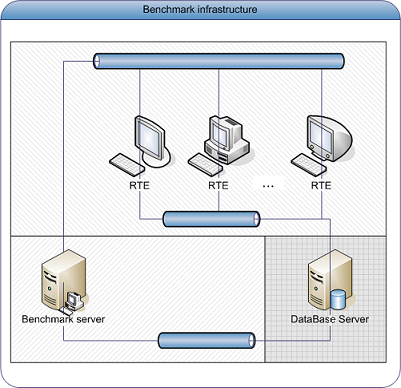
\includegraphics[width=0.6\linewidth]{figures/infrastructure.png}
\end{center}
\caption{Infrastruktura}\label{rys:infrastructure}
\end{figure}

\section{Test jako zestaw modeli}
Serwer benchmarku umożliwia ładowanie i uruchamianie testów. Każdy test składa się z trzech modeli (zob.~rys.~\ref{rys:models}):
\begin{itemize}
\item modelu bazy danych -- opisującego strukturę bazy danych, jak i populację danych w bazie przed rozpoczęciem testu,
\item modelu obciążenia -- opisującego obciążenie bazy danych. W skład tego modelu wchodzą: operacje, transakcje i użytkownicy,
\item modelu testu -- opisującego testowaną bazę danych, konfigurację połączenia do bazy, wartości parametrów skalujących 
powyższe modele, a także liczbę niezbędnych klientów RTE do przeprowadzenia testu.
\end{itemize}
\begin{figure}[h]
\begin{center}
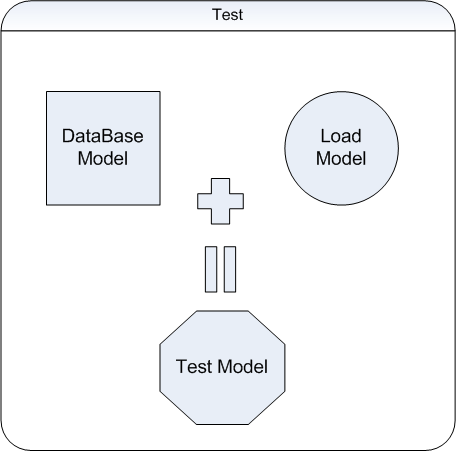
\includegraphics[width=0.4\linewidth]{figures/models.png}
\end{center}
\caption{Modele testu}\label{rys:models}
\end{figure}

\subsection{Model bazy danych}
Model bazy danych jest odpowiednikiem diagramu relacji, uzupełnionym o wartości 
liczby rekordów w poszczególnych relacjach (zob.~rys.~\ref{rys:database-model}). 
Wartości te mogą być określone względem parametru skalującego ,,n''. 
Konkretna wartość tego parametru jest określana w modelu testu. 
Liczba rekordów dla poszczególnych relacji jest wykorzystywana w procesie
generowania populacji bazy danych(zob. punkt~\ref{sect:populationgeneration}).
Warto podkreślić, iż opis zawarty w tym modelu jest niezależny od konkretnego DBMS 
(\english{Database Management System}). Formatem opisu modelu jest dokument XML,
dla którego zdefiniowano XMLSchema~\cite{XmlSchema1}, dostępną w załączniku do niniejszej pracy.
Przykładowy, uproszczony plik modelu bazy danych może wyglądać następująco:

\begin{codeblock}
<?xml version="1.0" encoding="UTF-8"?>
<database-model>
    <model-description/>
    <relations>
        <relation name="TBL_PERSON">
            <columns>
                <column name="ID" type="Long" is_id="true"/>
                <column name="FIRST_NAME" type="String(4,16)"/>
                <column name="SURNAME" type="String(4,32)"/>
                <column name="DATE_OF_BIRTH" type="Date"/>
            </columns>
        </relation>
    </relations>
    <population>
        <relation-population expression="1000*n" relation_name="TBL_PERSON"/>
    </population>
</database-model>
\end{codeblock}

W powyższym przykładzie zdefiniowano pojedynczą relację ,,TBL\_PERSON'', posiadającą
cztery atrybuty: ,,ID'', ,,FIRSTNAME'', ,,SURNAME'' oraz ,,DATE\_OF\_BIRTH''. Kolumna
,,ID'' jest kluczem głównym. Dla omawianej relacji określono niezbędną do wygenerowania 
populację początkową jako: ''1000*n'' -- oznacza to, iż liczba wygenerowanych rekordów
zależeć będzie od parametru skalującego ,,n'' i będzie od niego tysiąckrotnie większa.

\begin{figure}[h]
\begin{center}
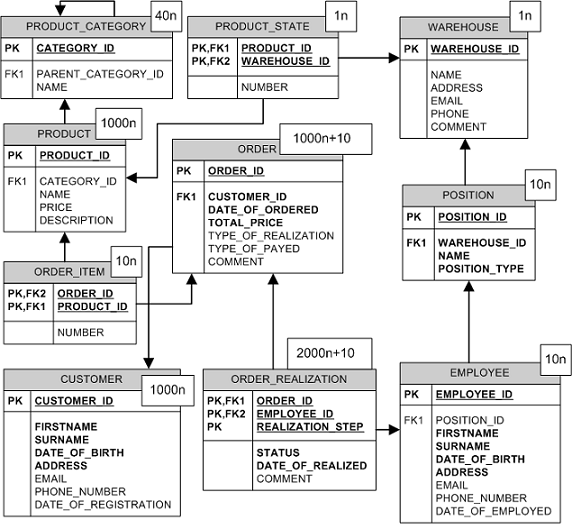
\includegraphics[width=0.9\linewidth]{figures/database-model.png}
\end{center}
\caption{Przykładowy model bazy danych}\label{rys:database-model}
\end{figure}

\subsection{Model obciążenia}
Model obciążenia(zob.~rys.~\ref{rys:load-model}) jest zmodyfikowaną wersją diagramu przypadków użycia z języka UML
(\english{Unified Modeling Language}, Ujednolicony Język Modelowania~\cite{UML1}~\cite{UML2}). Możemy tutaj wyróżnić 
użytkowników (aktorzy), a także transakcje i operacje (odpowiedniki przypadków użycia). Operacje to zwykłe operacje 
języka SQL(insert, update, delete, select).
Transakcje natomiast to zarazem transakcje w znaczeniu bazodanowym jak i odpowiedniki procesów biznesowych.
Transakcja jest uporządkowanym zbiorem krotności operacji, wchodzących w jej skład.
Istnieje możliwość określenia dla każdej transakcji minimalnej i maksymalnej liczby dla danego wystąpienia operacji.
Transakcje powodujące modyfikację zawartości bazy danych kończą się operacją ,,commit'', w przypadku wystąpienia
błędu w trakcie wykonywania którejś z operacji, transakcja kończy się operacją ,,rollback''.
Użytkownicy mogą wykonywać transakcje. Dla każdej transakcji, którą może wykonać dany użytkownik
należy podać średnią liczbę użycia na sesję. Dla każdego użytkownika podaje się czas trwania sesji,
a także liczbę użytkowników w systemie w jednostce czasu. Dany użytkownik może dziedziczyć
cechy po innym użytkowniku. Dziedziczenie może być pełne lub częściowe. Ilustruje to poniższy rysunek.

\begin{figure}[h]
\begin{center}
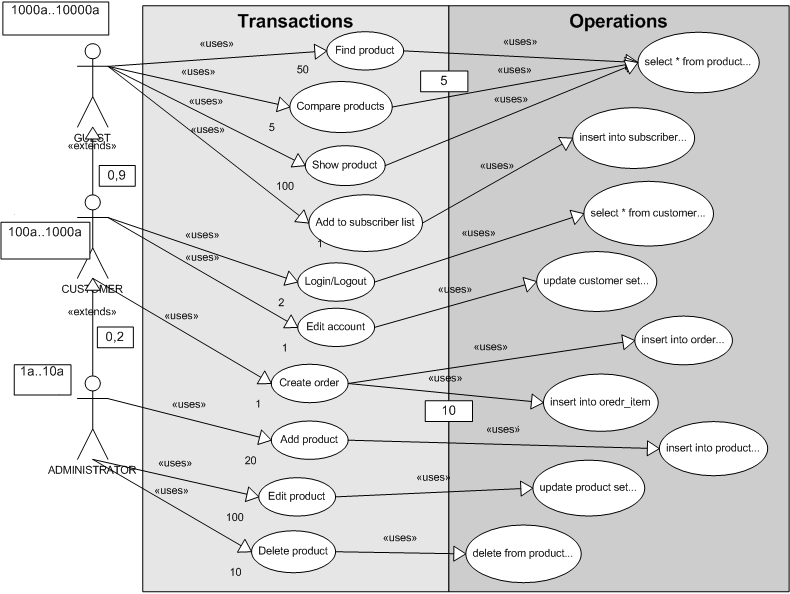
\includegraphics[width=1.0\linewidth]{figures/load-model.png}
\end{center}
\caption{Przykładowy model obciążenia}\label{rys:load-model}
\end{figure}
Widzimy tutaj min., iż transakcja ,,Create order'' składa się z dwóch typów operacji: ,,insert into order'' 
oraz ,,insert into order\_item''. Pierwsza operacja jest wykonywana w transakcji 1 raz, druga zaś 10 razy.
Użytkownik ,,Customer'' wykonuje w trakcie jednej sesji 2 transakcje ,,Login/Logout'', 1 transakcje ,,Edit account'',
oraz jedną ,,Create order''. Użytkownik ten dziedziczy również transakcje po użytkowniku ,,Guest''. Stopień dziedziczenia
określia liczba ,,0.9'' umieszczona obok strzałki od użytkownika ,,Customer'' do ,,Guest''. Oznacza to, iż 
,,Customer'' wykonuje 0.9 tych samych transakcji co ,,Guest'', czyli np. $0.9 * 100$ transakcji ,,Show product''.
W rozważanym przedziale czasu w systemie może przebywać od 100a do 1000a użytkowników typu ,,Customer''. Podczas wykonywania testów
przyjęta zostanie wartość średnia czyli 550a. 

Wszystkie powyższe cechy umożliwiają dużą elastyczność w budowie modelu obciążenia bazy danych.
Dodatkowo parametry takie, jak liczba użytkowników( parametr ,,a'') mogą być skalowane. 
Podobnie jak dla modelu bazy danych formatem opisu jest dokument XML,
dla którego zdefiniowano XMLSchema, dostępną w załączniku do niniejszej pracy.
Przykładowy, uproszczony plik modelu obciążenia może wyglądać następująco:

\begin{codeblock}
<?xml version="1.0" encoding="UTF-8"?>
<load-model>
    <description>Typowy model sklepu</description>
    <operations>
        <operation name="INSERT INTO TBL_PERSON" type="INSERT">
            <definition>INSERT INTO TBL_PERSON(FIRST_NAME,SURNAME,DATE_OF_BIRTH) 
	    		VALUES(?,?,?)</definition>
            <operation-description>Wstawienie nowego rekordu do tabeli użytkownicy</operation-description>
            <parameters>
                <parameter type="String(4,16)" number="1"/>
                <parameter type="String(4,32)" number="2"/>
                <parameter type="Date" number="3"/>
            </parameters>
        </operation>
    </operations>
    <transactions>
        <transaction name="ADD PERSON">
            <transaction-description>Add new person</transaction-description>
            <transaction-operations>
                <transaction-operation operation_name="INSERT INTO TBL_PERSON" number="1"/>
            </transaction-operations>
        </transaction>
    </transactions>
    <actors>
        <actor min_number="1*a" max_number="100*a" name="ADMIN">
            <actor-description/>
            <actor-transactions>
                <actor-transaction transaction_name="ADD PERSON" avg_call_number="100"/>
            </actor-transactions>
        </actor>
    </actors>
</load-model>
\end{codeblock}
W powyższym przykładzie zdefiniowano pojedyńczą operację ,,INSERT INTO TBL\_PERSON'',
operacja ta wstawia nowy rekord do tabeli ,,TBL\_PERSON''. Sama operacja jest typową operacją INSERT
z języka SQL, w miejscach wstawianych wartości umieszczono znaki ,,?''. Konkretne wartości są bowiem generowane
podczas tworzenia skryptów testowych. Typy generowanych wartości dla danej operacji określa się w sekcji
,,parameters''. W zamieszczonym przykładzie zdefiniowano również jedną transakcję ,,ADD PERSON''.
Transakcja ta składa się z pojedynczego wywołania operacji ,,INSERT INTO TBL\_PERSON''.
Ostatnim elementem zdefiniowanym w omawianym przykładzie jest aktor ,,ADMIN'',
reprezentuje on użytkownika typu administrator. Użytkownik ten wykonuje średnio
100 transakcji ,,ADD PERSON''.
Liczba administratorów w systemie waha się od 1*a do 100*a, gdzie ,,a'' jest parametrem skalującym dla aktorów.
Parametr ten określa się w modelu testu. Podczas testów brana jest pod uwagę średnia liczba administratorów 
czyli dla powyższego przykładu 50,5*a, przy czym po ustaleniu wartości a, liczba ta jest zaokrąglana w dół
do liczby całkowitej.

\subsection{Model testu}\label{sect:testmodel}
Model testu wiąże model bazy danych i model obciążenia. Określa on:
\begin{itemize}
\item wartości parametrów skalujących (,,a'', ,,n'', ,,c''), 
\item liczbę klientów RTE potrzebnych do wykonania testu, 
\item parametry połączenia z bazą danych, 
\item sterownik JDBC, 
\item a także, czy baza danych ma zostać usunięta po zakończeniu testu. 
\end{itemize}

To właśnie w tym modelu, poprzez specyfikacje dialektu, następuje określenie typu DBMS. 
Na podstawie zaś dialektu, w procesie przygotowywania danych, modele te są odpowiednio interpretowane.
Model ten udostępnia duże możliwości skalowalności, poszczególne parametry skalujące
mają określone zastosowanie:
\begin{itemize}
\item ,,a'' -- służy  do określania liczby użytkowników w modelu obciążenia,
\item ,,n'' -- przeznaczeniem tego parametru jest określanie liczby rekordów dla generowania populacji, w modelu bazy danych, 
\item ,,c'' -- jest parametrem wiążącym pozostałe 4 parametry, może być używany w ich definicji,
dzięki niemu można uzyskać pojedynczy parametr skalujący dla testu.
\end{itemize}
Poniżej przedstawiono przykładowy model testu:
\begin{codeblock}
<?xml version="1.0" encoding="UTF-8"?>
<test-model delete_db_after_test="false" rte_number="2" c="4" n="2000* c" a="1000*c">
	<jdbc-connection-properties>
		<property name="jdbc-library-location" value="/jar/jdbc.jar"/>
		<property name="driver_class" value="com.mysql.jdbc.Driver"/>
		<property name="dialect" value="MySQLInnoDBDialect"/>
		<property name="url" value="jdbc:mysql://localhost:3306/test"/>
		<property name="username" value="root"/>
		<property name="password" value=""/>
	</jdbc-connection-properties>
</test-model>
\end{codeblock}

W definicjach poszczególnych parametrów (,,a'', ,,n'') oraz w miejscach ich wstawiania w modelach, można
użyć operatorów ,,$+$'', ,,$-$'', ,,$*$'', ,,$:$'', ,,$^{\wedge}$'' (potęgowanie), a także funkcji ,,ln'' i ,,log'' oraz
nawiasy ,,('', ,,)''. Operacje są wykonywane w kolejności występowania od lewej do prawej tzn.
wszystkie operatory mają równy priorytet. Poprawne są zatem w definicjach modeli konstrukcje takie jak ,,$(n+((5+n)*n)):2*n$''
w miejscu dozwolonym dla parametru ,,n'' i~analogicznie dla~,,a''.
W samym modelu testu w~definicjach parametrów ,,a'' oraz~,,n'',
stosować można wyłącznie odwołania do parametru c tzn. poprawna jest definicja 
n="$2*c+1$", a niepoprawna n="$3*a$". Przykładowa definicja wszystkich parametrów
w modelu testu może wyglądać np. tak: c="1", a="2 $^{\wedge} c$", n="$100 * c + 10$".

\section{Podsumowanie}
Podział definicji testu na trzy modele, ułatwia zdefiniowanie testu. Każdy model 
ma ściśle określone przeznaczenie, razem zaś stanowią pełną definicję, 
uwzględniającą wszystkie aspekty rzeczywistego systemu opartego o współpracę z DBMS. 
Takie podejście ułatwia definiowanie testu, zmiana DBMS sprowadza się do zmiany dialektu 
i~parametrów połączenia w modelu testu. Koncepcja taka zapewnia również łatwą, 
wielokryterialną skalowalność.


\chapter{Przygotowanie danych}
Przeprowadzenie procedury testu wiąże się z czynnościami mającymi charakter przygotowawczy. 
Należy do nich min.:
\begin{itemize}
\item stworzenie relacji bazy danych,
\item wypełnienie relacji danymi początkowymi tzw. populacją bazy danych,
\item przygotowanie skryptów testowych.
\end{itemize}
W stworzonym benchmarku operacje te zostały zgrupowane razem w etapie zwanym ,,przygotowanie danych''. 
Niniejszy rozdział omawia ten właśnie etap.
\section{Tworzenie relacji bazy danych}
Jak już zostało wspomniane, model bazy danych jak i model obciążenia, są niezależne
od konkretnego DBMS. Pierwszym momentem, w którym następuje związanie tych modeli
z konkretnym DBMS, jest właśnie moment tworzenia relacji w bazie danych.
Pomimo istnienia języka SQL poszczególne DBMS różnią się pomiędzy sobą dostępnymi typami danych.
Typy te są szczególnie widoczne w zapytaniach tworzących relacje. W omawianym benchmarku
do tworzenia skryptów tworzących relacje została użyta biblioteka Hibernate~\cite{Hibernate1} 
oraz Hibernate Annotations~\cite{HibernateAnn1}.
Proces tworzenia relacji składa się z następujących etapów:
\begin{enumerate}
\item Wygenerowanie na podstawie modelu bazy danych klas -- zgodnych ze
specyfikacją Hibernate Annotations.
\item Kompilacja klas.
\item Załadowanie klas do biblioteki Hibernate. 
\item Wygenerowanie skryptów przy pomocy biblioteki Hibernate.
\item Utworzenie relacji w bazie danych.
\end{enumerate}
\section{Generowanie populacji bazy danych}\label{sect:populationgeneration}
Aby móc przeprowadzić testy na bazie danych niezbędne jest by w bazie tej znajdowały się dane.
Dane te powinny charakteryzować się szeregiem własności:
\begin{itemize}
\item odpowiednią proporcją pomiędzy liczbą krotek w poszczególnych relacjach,
\item odpowiednią zawartością wartości pustych w poszczególnych kolumnach,
\item monotonicznością lub jej brakiem dla poszczególnych atrybutów,
\item zakresem dopuszczalnych wartości np.: w przypadku typów wyliczeniowych, czy kluczy obcych.
\end{itemize}
Na podstawie informacji z modelu bazy danych, oraz wartości parametrów skalujących z modelu 
testu, relacje bazy danych wypełniane są krotkami. Proces ten w ogólności nie jest trywialny -- 
powstaje tutaj szereg problemów, jak chociażby generowanie złożonych kluczy głównych, 
czy złożonych kluczy obcych. Już samo istnienie referencji na inne relacje wymusza uszeregowanie relacji np.: 
aby wprowadzić wartość dla klucza obcego w relacji A, muszą istnieć dane w relacji B.

Algorytm tworzenia populacji
\begin{enumerate}
\item Uszereguj relacje -- postępuj zgodnie z algorytmem poszukiwania cykli w grafie.
(Kolejność usuwania relacji w algorytmie jest kolejnością posortowania relacji.)
Mechanizm tworzenia populacji benchmarku, nie radzi sobie z cyklami -- poza cyklami na ,,siebie''.
Cykl na ,,siebie'' jest to klucz obcy na własne kolumny. Przykładem cyklu z jakim mechanizm sobie nie radzi,
może być cykl pomiędzy trzema relacjami A, B i C, gdzie relacja A posiada klucz obcy na B, B na C oraz C na A. 
Warto jednak zauważyć, że istnienie zależności cyklicznych zarówno w programowaniu obiektowym, 
jak i w bazach danych, jest przykładem złej praktyki. Praktycznie każdą zależność cykliczną 
idzie przekształcić na zależność jednokierunkową.

\item Utwórz generatory krotek relacji.
\item Wyszukaj wszystkie kolumny każdej relacji używane jako klucze obce -- w ten sposób określa się, 
które kolumny mają mieć wartości generowane na podstawie wartości innych kolumn. Jeżeli bowiem kolumna
jest kluczem obcym na inną kolumnę, to jej wartości muszą pochodzić z tej właśnie kolumny.
\item Utwórz struktury buforujące dla poszczególnych relacji/generatorów relacji.
\item Ustaw klucze obce w generatorach relacji.
\item Generuj dane.
\end{enumerate}
\section{Przygotowanie skryptów testowych}
\subsection{Wstęp}
Ważnym etapem przygotowywania danych jest utworzenie skryptów testowych, które następnie
w procedurze testu będą wykonywane na poszczególnych RTE. Liczba potrzebnych skryptów
jest równa liczbie RTE niezbędnych w procedurze testu. Dla każdego skryptu,
na podstawie analizy modelu obciążenia, a także parametrów skalujących z modelu testu, 
określana jest liczba operacji i transakcji do przetestowania na pojedynczym RTE.
Następnie dla każdego RTE tworzony jest niezależnie skrypt testowy –- o tej samej strukturze, 
lecz różnych danych, dla poszczególnych operacji.
\subsection{Budowa skryptu testowego}\label{sub:testscript}
Na rys.~\ref{rys:test-script} przedstawiono przykładowy skrypt testowy przeznaczony do wykonania na jednym z RTE. 
Rzeczywisty skrypt jest oczywiście bardziej złożony, posiada min.: wielokrotnie więcej operacji SQL. 
Rzeczywisty skrypt generowany jest dla każdego RTE przez serwer, przed rozpoczęciem testu.
Zawiera on zestaw testów dla poszczególnych operacji i transakcji opisanych w modelu obciążenia. Każda 
komenda ,,nie SQL'' poprzedzona jest znakiem ,,$>$''. Poniżej wyjaśniono wszystkie te komendy:
\begin{itemize}
\item $>$s -- wysłanie z RTE sygnału synchronizującego do serwera, serwer oczekuje na sygnały synchronizujące od
wszystkich RTE biorących udział w teście, po czym odsyła do nich własny sygnał synchronizujący,
\item $>$w -- oczekiwanie przez klienta RTE na sygnał synchronizujący z serwera, dalsze wykonywanie skryptu testowego jest
zawieszane,
\item $>$t -- pomiar czasu na RTE i zapisanie go do pliku ,,test.time'',
\item $>$c -- wykonanie operacji commit,
\item $>$l -- wykonanie operacji SQL wymagającej wstawienia obiektu typu LOB(\english{large object}) 
czyli BLOB (\english{binary large object}) lub CLOB (\english{character large object}). 
Obiekty tego typu nie są umieszczane bezpośrednio w skrypcie, lecz w 
dwóch odrębnych plikach ,,test.blob'' oraz ,,test.clob''. Interpreter skryptu, 
gdy napotka komendę rozpoczynającą się od litery~,,l'' analizuje ją do pierwszego znaku~,,:''. 
Znakiem ,,,'' rozdzielone są sekcje dotyczące kolejnych obiektów lob. 
Pierwsza litera każdej sekcji ,,mówi'' czy sekcja dotyczy obiektu typu BLOB czy CLOB. 
Każda sekcja zawiera także informacje o długości obiektu. Kolejność sekcji odpowiada kolejności
występowania odwołań do obiektów lob w komendzie języka SQL, umieszczonej po pierwszym znaku~,,:''. 
Miejsca, w których obiekty te mają się znaleźć oznaczone są znakiem~,,?''. 
W zależności od typu sterownika wstawianie obiektów LOB odbywa się albo poprzez funkcje 
,,setBinaryStream'', ,,setCharacterStream'' lub ,,setBlob'', ,,setClob''.
\end{itemize} 

\begin{figure}[t]
{\footnotesize
$>$s /*Wysłanie sygnału do serwera*/\\
$>$w /*Oczekiwanie na sygnał z serwera*/\\
$>$t /*Pomiar czasu*/\\
select * from tbl\_customer where customer\_id = 12\\
$>$t \\
$>$s \\
$>$w \\
$>$t \\
insert into tbl\_subscriber(email) values('janek@wp.pl')\\
$>$t \\
$>$r /*Operacja rollback*/\\
$>$t \\
update tbl\_person set sex = 'male‘ where person\_id = 7\\
delete from tbl\_subscriber where email = 'mirek@wp.pl'\\
$>$t\\
$>$s\\
$>$w\\
$>$t\\
l,b1200,c123:insert into tbl\_products values('name',?,?)\\
$>$t\\
$>$c /*Operacja commit*/\\
$>$s\\ 
}
\caption{Przykładowy skrypt testowy}\label{rys:test-script}
\end{figure}
Na uwagę zasługuje fakt, iż para operacji ,,$>$s $>$w'' występuje poza wysłaniem ostatniego sygnału 
synchronizującego do serwera, zawsze razem. Pierwsza operacja powoduje wysłanie z RTE sygnału 
synchronizującego do serwera, druga zaś wstrzymuje wykonanie testu do momentu wysłania sygnału 
synchronizującego w odwrotnym kierunku. Serwer odsyła każdorazowo taki sygnał, gdy otrzyma 
sygnały synchronizujące od wszystkich RTE biorących udział w teście. Taki zabieg umożliwia synchronizację 
wykonywanych na poszczególnych RTE skryptów testowych. Synchronizacja taka jest wykonywana 
przed każdym testem. Po zakończeniu testu, każdy RTE wysyła do serwera ostatni sygnał synchronizujący, 
gdy serwer otrzyma taki sygnał od każdego RTE –- ,,wie'', że procedura testowa zakończyła się.
Ponadto, jeżeli w trakcie wykonywania którejś z komend języka SQL wystąpi wyjątek, to zostanie 
on przechwycony i zapisany w pliku ,,test.error'', wraz z numerem linii skryptu, którego błąd dotyczył. 
Zamieszczone w przykładzie komentarze typu /*…*/ w rzeczywistym skrypcie nie występują. 
\subsection{Typy testów}\label{sect:testtypes}
Skrypt testowy składa się z czterech typów testów:
\begin{itemize}
\item obciążeniowego operacji,
\item obciążeniowego transakcji,
\item proporcjonalnościowego operacji,
\item proporcjonalnościowego transakcji.
\end{itemize}

Testy obciążeniowe operacji to testy, w których występują operacje zdefiniowane w modelu obciążeniowym.
Podczas tego typu testów na wszystkich RTE równocześnie wykonywane są operacje \textit{tylko} jednego typu.
Testy takie pozwalają przyjrzeć się dokładnie jednemu typowi operacji, nie uwzględniają jednak całej złożoności
modelu obciążeniowego.

Testy obciążeniowe transakcji to testy, w których na wszystkich RTE równocześnie wykonywane są transakcje \textit{tylko} jednego typu.
Testy takie pozwalają przyjrzeć się dokładnie jednemu typowi transakcji, nie uwzględniają jednak całej złożoności
modelu obciążeniowego.

Testy proporcjonalnościowe operacji to testy, w których na wszystkich RTE równocześnie wykonywana jest pewna 
,,proporcjonalnościowa mieszanka'' operacji. Na każdym RTE kolejność operacji jest losowa, proporcjonalność zaś
wynika z obliczeń dokonywanych na podstawie modelu obciążeniowego.

Testy proporcjonalnościowe transakcji to testy, w których na wszystkich RTE równocześnie wykonywana jest pewna 
,,proporcjonalnościowa mieszanka'' transakcji. Na każdym RTE kolejność transakcji jest losowa, proporcjonalność zaś
wynika z obliczeń dokonywanych na podstawie modelu obciążeniowego.

\subsection{Podsumowanie}
Reasumując, w procedurze generowana skryptów testowych, dla każdego RTE biorącego 
udział w teście zostają wygenerowane trzy pliki: ,,test.script'', ,,test.blob'' oraz ,,test.clob''.
Pliki te wraz ze sterownikiem jdbc (,,jdbc.jar''), a także z opisem parametrów połączenia i dialektem (plik ,,test.properties''), 
pakowane są do archiwum ,,test.zip'' (zob. rys.~\ref{rys:testzip}). Ostatecznie otrzymujemy kolekcje plików zip 
–- po 1 na każdego klienta RTE, który ma wziąć udział w teście.
\begin{figure}[h]
\begin{center}
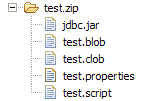
\includegraphics[width=0.4\linewidth]{figures/testzip.png}
\end{center}
\caption{Struktura pliku ,,test.zip''}\label{rys:testzip}
\end{figure}
Ostatnim etapem generacji skryptów testowych jest wygenerowanie pliku ,,test.metadata''. 
Plik ten zawiera informacje dla serwera niezbędne w procesie zbierania i analizy wyników testu.
Plik ten nie jest wysyłany do RTE, serwer przechowuje go lokalnie u siebie. 




\chapter{Procedura testu}
Rozdział ten omawia wszystkie aspekty związane bezpośrednio z przeprowadzaniem procedury testu.
W jej skład wchodzi: dystrybucja aplikacji RTE na poszczególne komputery pomiarowe,
zestawianie połączeń serwer -- klienci RTE, dystrybucja testów, przeprowadzanie procedury testu
oraz zbieranie wyników pomiarów.

\section{Dystrybucja RTE}
Niniejszy benchmark jest aplikacją typu klient -- serwer. Rolę klientów pełni w niej aplikacja
RTE, która służy bezpośrednio do wykonywania testów. Aplikacja ta jest uruchamiana na wielu komputerach,
w związku z tym powstaje problem jej dystrybucji. Problem ten został rozwiązany poprzez rozszerzenie
funkcjonalności serwera benchmarku, o funkcjonalność serwera ftp, udostępniającego do pobrania aplikację RTE. 
A zatem, na każdym komputerze na, którym planowane jest zainstalowanie RTE, wystarczy użyć 
klienta ftp, połączyć się z serwerem benchmarku, a następnie pobrać i rozpakować aplikację.

\section{Tworzenie infrastruktury klient -- serwer}\label{sect:infra}
Komunikacja klient -- serwer została oparta o protokół RMI oraz wsparcie oferowane
mu przez framework Spring 2.0. Niezbędne jest zatem odblokowanie odpowiednich portów,
by komunikacja była możliwa. Standardowo serwer RMI benchmarku nasłuchuje na porcie 1199,
klienci RTE mają natomiast przydzielane numery portów dynamicznie tzn. pierwszy wolny port
większy od 1024. Uruchomienie klienta RTE jest możliwe tylko i wyłącznie, gdy serwer RMI benchmarku
jest uruchomiony i dostępny. Przed rozpoczęciem właściwej procedury testu należy zatem uruchomić
serwer benchmarku i wymaganą liczbę klientów RTE. 

Uruchomienie klienta RTE sprowadza się do dwóch czynności:
\begin{enumerate}
\item Wyedytowania, znajdującego się w głównym katalogu klienta -- pliku ,,rte-config.xml''.
Plik ten wygląda następująco:
\begin{codeblock}
<?xml version="1.0" encoding="UTF-8"?>
<rte-config>
	<server-rmiserver>rmi://HOST_NAME:1199/JDBMeasureRMIServer</server-rmiserver>
</rte-config>
\end{codeblock}
Należy w nim zamienić ciąg znaków ,,HOST\_NAME'' na nazwę lub adres IP serwera testu.
Istnieje również możliwość zmieniany numeru portu ze standardowego 1199 --  z tej opcji należy jednak korzystać
jedynie w sytuacji, gdy serwer benchmarku korzysta z innego portu niż standardowy.
\item Wykonać z lini poleceń (w katalogu głównym klienta RTE) następującą komendę: 
\begin{Verbatim}
java -jar rte.jar
\end{Verbatim}
Zarówno klient RTE jak i aplikacja serwera wymagają do pracy zainstalowania na
komputerze JVM (\english{Java Virtual Machine }~\cite{JVM1}),
w wersji 1.5 lub wyższej.
\end{enumerate}
Na pojedynczym hoście można uruchomić wiele instancji klienta RTE, ponadto nic nie stoi na przeszkodzie
by klient taki znajdował się na komputerze, na którym uruchomiony jest serwer benchmarku.
Takie rozwiązanie nie jest zalecane w sytuacji, gdy serwer benchmarku generuje zauważalne obciążenie
podczas procedury testu, gdyż przekładało by się ono na wyniki pomiarów z RTE. Jeżeli procedura 
uruchamiania wymaganych klientów RTE przebiegnie pomyślnie, infrastruktura testu jest gotowa do użycia.

Warto jest w tym miejscu przyjrzeć się bliżej infrastrukturze benchmarku (zob. rys.~\ref{rys:infrastructure2b}).
\begin{figure}[h]
\begin{center}
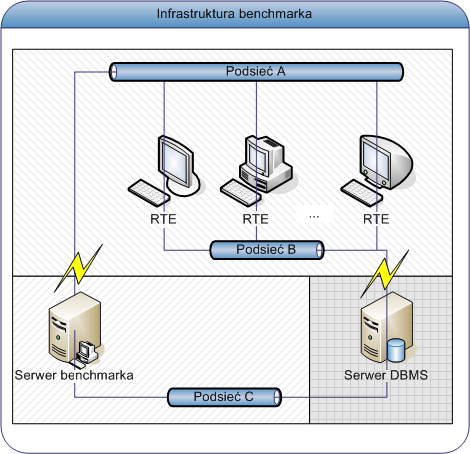
\includegraphics[width=0.8\linewidth]{figures/infrastructure2b.png}
\end{center}
\caption{Infrastruktura benchmarku}\label{rys:infrastructure2b}
\end{figure}
Składa się ona z trzech segmentów/podsieci. Na etapie przygotowywania danych
wykorzystywana jest podsieć C, podsieci A i B nie są wówczas w ogóle potrzebne.
Natomiast podczas procedury testu sytuacja się odwraca -- wówczas to serwer benchmarku
nie komunikuje się bezpośrednio z bazą danych. Warto również zauważyć, iż komunikacja w podsieciach B i~C
odbywa się za pomocą sterowników JDBC, natomiast w sieci A wykorzystywane są protokoły~RMI oraz~ftp.
Podczas inicjalizowania i~finalizowania procedury testu główne obciążenie generowane jest w podsieci~A
ze względu na przesyłanie: klientów RTE, danych testowych i rezultatów testów. W samej zaś procedurze testu
główny ruch przypada na podsieć B. To właśnie ta podsieć, jej parametry techniczne i obciążenie wpływają na 
jakość uzyskiwanych wyników.

\section{Przekazanie skryptów testowych}
Klienci RTE bezpośrednio po połączeniu z serwerem, oczekują na przekazanie skryptów testowych
i zainicjalizowanie procedury testu. W pierwszym kroku serwer przekazuje każdemu RTE
przeznaczonemu do udziału w procedurze testowej -- archiwum ,,test.zip''. Każdy RTE otrzymuje (sekwencyjnie)
inne archiwum ,,test.zip''. RTE po pobraniu archiwum, rozpakowuje je. Następnie ładuje sterownik 
JDBC do bazy danych, testuje połączenie, otwiera strumienie do plików wejściowych i wyjściowych. 
Po pomyślnym wykonaniu powyższych czynności przechodzi w tryb oczekiwania na komendę rozpoczęcia testu.

\section{Wykonywanie testów}
Bezpośrednie wykonywanie testów, rozpoczęcie procedury testu -- następuje po przekazaniu
przez serwer, sygnału synchronizacyjnego -- wszystkim klientom RTE wyznaczonym do udziału w procedurze.
W tym momencie rozpoczyna się zasadnicza procedura testu.

Następnie następuje sekwencja operacji, w której każdy RTE biorący udział w procedurze testowej,
wysyła sygnał synchronizujący do serwera i oczekuje na odesłanie podobnego sygnału synchronizującego. 
Serwer odsyła taki sygnał, gdy otrzyma  sygnały synchronizujące od wszystkich RTE biorących udział w procedurze testowej.
Pomiędzy parami przesłań sygnałów synchronizujących, każdy RTE wykonuje testy, 
zapisując czasy i przechwycone błędy do plików ,,test.time'' oraz ,,test.error''.
Po zakończenia wszystkich testów, każdy RTE wysyła ostatni sygnał synchronizujący. 
Gdy serwer otrzyma ten sygnał od wszystkich RTE ,,wie'', że procedura testu dobiegła końca.
	
Omówione powyżej sygnały synchronizujące są ważnym elementem procedury testu (zob. także punkt~\ref{sub:testscript}). 
To dzięki nim testy składowe zawarte w skryptach wykonywanych na poszczególnych RTE,
są zsynchronizowane -- oznacza to, że niezależnie od różnych czasów zakończenia danego testu,
kolejny test składowy nie rozpocznie się przed zakończeniem, aktualnego testu na wszystkich RTE.

\section{Zbieranie wyników}
Po zakończeniu procedury testu, z każdego RTE biorącego w  niej udział, serwer pobiera poprzez protokół RMI, 
plik ,,testresult.zip''(zob. rys.~\ref{rys:testresultzip}).
\begin{figure}[h]
\begin{center}
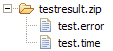
\includegraphics[width=0.3\linewidth]{figures/testresultzip.png}
\end{center}
\caption{Struktura pliku ,,testresult.zip''}\label{rys:testresultzip}
\end{figure}
Plik taki zawiera czasy zarejestrowane podczas procedury, jak i błędy wykonania
operacji na bazie danych. Raz zebrane wyniki mogą być następnie analizowane wielokrotnie
przez serwer benchmarku. Przy czym do analizy takiej, nie jest już wymagane połączenie
z klientami RTE.

\section{Podsumowanie}
Procedura testu składa się zasadniczo z wykonywania przez RTE skryptów testowych,
mierzenia czasów i wymiany sygnałów synchronizujących z serwerem. Wydawałoby się zatem, 
iż nie jest to etap złożony. Należy jednak pamiętać, iż prawidłowość procedury testu
nie sprowadza się jedynie do wykonania wyżej omówionych kroków. Przed rozpoczęciem procedury
testu należy zminimalizować wpływ na wyniki czynników zewnętrznych tj.:
\begin{itemize}
\item Nadmiernego obciążenia sieci i zbyt dużych czasów komunikacyjnych w podsieci B (zob. rys.~\ref{rys:infrastructure2b}).
W procedurze testu należy zatem tak dobrać hosty na, których mają działać aplikacje RTE,
by wpływ tych czynników był jak najmniejszy. Sam benchmark nie niweluje wpływu przepustowości
sieci. Wpływ ten może mieć charakter statyczny -- wynikający z architektury sieci jak i dynamiczny
-- zależny od obciążenia wykorzystywanych segmentów sieci. Nie zaleca się zatem przeprowadzania
testów przez sieć rozległą np.: Internet.
\item Obciążenia przez inne oprogramowanie hostów wykorzystywanych w procedurze testu.
Główną przyczyną jest tutaj dłuższy czas oczekiwania na przydział zasobów tj.: 
dysk twardy, pamięć RAM, karta sieciowa, czas procesora itp.
\item Wykorzystywania DBMS podczas testu przez inne aplikacje.
\end{itemize}
Dopiero uwzględnienie tych czynników w połączeniu z poprawnie wykonaną procedurą testu,
daje w rezultacie istotne dane. 

Korzystając z benchmarku można jednak spróbować oszacować wpływ czynników zewnętrznych 
na wydajność bazy danych widzianą z punktów pomiarowych (hostów RTE). Taki eksperyment
może mieć sens dla konkretnej, istniejącej sieci. W tym celu należy przeprowadzić test dwukrotnie: 
raz w systemie ze zniwelowanym wpływem czynników zewnętrznych, drugi raz w systemie/sieci 
pracującym przy typowym obciążeniu, generowanym przez inne aplikacje. 
Porównując wyniki obu testów można wyciągnąć wnioski,
na które testowane operacje/transakcje zauważalny wpływ mają czynniki zewnętrzne.
Z powyższego eksperymentu może się bowiem okazać, iż ,,wąskim gardłem'' jest 
istniejąca infrastruktura sieci, a nie DBMS, czy testowana baza danych.




\chapter{Analiza wyników testu}\label{chap:testresultanalysis}
Rozdział ten omawia analizę zebranych wyników z przeprowadzonej procedury testu.
Na uwagę zasługuje fakt, iż analiza może zostać dokonana w dowolnym momencie po zakończeniu testów,
tzn.: nie jest wymagane istnienie połączeń klientów RTE. Wszystkie wyniki bowiem po zakończeniu testu,
są przekazywane na serwer i tam pamiętane.
\section{Analiza}
Jak już wspomniano, ostatnim etapem testowania jest analiza wyników procedury testu. 
Analiza ta jest wykonywana na podstawie:
\begin{itemize}
\item zawartości plików ,,testresult.zip'' uzyskanych z RTE biorących udział w testach,
\item zawartości pliku ,,test.metadata'',
\item analizy modelu obciążenia,
\item wartości parametrów skalujących opisanych w modelu testu,
\item liczby RTE biorących udział w procedurze testowej.
\end{itemize}
Efektem analizy dokonanej przez serwer jest wygenerowanie raportu tekstowego
oraz histogramów czasów odpowiedzi.
\section{Generowanie raportu}\label{sect:textraport}
Raport z testu obejmuje cztery typy testów omówione w punkcie \ref{sect:testtypes}.
Typy te dzielą raport na cztery sekcje:
\begin{enumerate}
\item Wyniki testu obciążeniowego operacji,
\item Wyniki testu obciążeniowego transakcji,
\item Wyniki testu proporcjonalnościowego operacji,
\item Wyniki testu proprocjonalnościowego transakcji.
\end{enumerate}
W sekcji 1 wymienione są wszystkie operacje zdefiniowane w modelu obciążeniowym
w kolejności od operacji najbardziej kosztownej do najmniej. Dla każdej operacji 
podano szereg właściwości:
\begin{itemize}
\item liczbę operacji przypadających na pojedynczy RTE,
\item liczbę wszystkich operacji,
\item średni czas wykonania wszystkich operacji na pojedynczym RTE -- jest to czas
wykonania operacji przydzielonych dla pojedynczego RTE,
\item medianę dla tego czasu,
\item standardowe odchylenie tego czasu,
\item oraz średni czas wykonania pojedynczej operacji.
\end{itemize}
Przykładowy fragment raportu tekstowego z tej sekcji może wyglądać następująco:
\begin{codeblock}
*********************************************************************************
Operation name: SELECT FROM TBL_PRODUCT
Operation type: SELECT
Operation definition:  SELECT * FROM TBL_PRODUCT WHERE PRICE >= ? AND PRICE <= ? AND CATEGORY_ID = ?
Operation description: Wyszukiwanie produktów po cenie i kategorii

Number of test operations per RTE:  5162
Total number of test operations:    41296

Avarage RTE time:               22s 18ms 457us
Median RTE time:                25s 53ms 151us
Standard deviation RTE time:    6s 550ms 933us

Single operation time avarage:  4ms 265us
*********************************************************************************
\end{codeblock}
,,Single operation time avarage'' jest średnim czasem wykonania pojedynczej operacji, czas ten nie jest jednak zmierzony,
lecz wyliczony. Wynika to z faktu, iż dla testów obciążeniowych czasy mierzone są przed rozpoczęciem i po zakończeniu
bloku operacji. Dzięki temu uzyskano większe obciążenie bazy danych. ,,Avarage RTE time'' jest średnim czasem wykonania na RTE
bloku operacji.

%Dla tego typu testów ze względu na liczbę operacji, czas nie jest mierzony dla pojedynczej operacji, a dla grupy operacji
%na pojedynczym RTE, w związku z tym nie możemy wyznaczyć wariancji, mediany czy odchylenia standardowego
%dla średniego czasu wykonania pojedynczej operacji. 
%Czas ten nie jest mierzony ze względu na minimalny 
%czas trwania pojedynczej operacji, w stosunku do którego błąd pomiaru jest znaczący. 
%Podczas pomiaru czasu
%należy bowiem uwzględnić szereg czynników takich jak występowanie wątków i procesów pomiędzy, którymi system operacyjny jest
%przełączany, a na który bezpośrednio nie mamy wpływu w systemie wielozadaniowym. 

%Rozważmy pewien przykład: załóżmy, że testom zostaje poddanych $n = 1000$ operacji, 
%przy pomiarze czasu oddzielnie dla każdej operacji otrzymujemy 1000 wyników, 
%każdy wynik obarczony jest pewnym błędem $\bigtriangleup_i$. Oznaczmy rzeczywisty czas trwania operacji
%przez $t_i$. Jeżeli $t_i \approx \bigtriangleup_i$ to $\sum_{i=1}^n(\bigtriangleup_i + t_i) \neq \sum_{i=1}^n(t_i)$.
%Tylko w sytuacji, gdy $t_i \gg \bigtriangleup_i$ to $\sum_{i=1}^n(\bigtriangleup_i + t_i) \approx \sum_{i=1}^n(t_i)$.
%Widzimy zatem, iż w sytuacji, gdy mierzony czas jest bliski granicy błędu należy stosować pomiar grupowy,
%w takiej sytuacji mamy pojedynczy czas $\sum_{i=1}^n(t_i) + \bigtriangleup$, gdzie $\bigtriangleup$ to
%błąd pomiaru. 

%Innym powodem wyboru tej metody pomiarowej dla testów obciążeniowych była chęć wygenerowania
%możliwie jak największego obciążenia. Pomiar czasów przed i po każdej operacji, na każdym RTE
%powodowałby chwilowe zmniejszenie obciążenia DBMS.

W sekcji 2 wymienione są wszystkie transakcje zdefiniowane w modelu obciążeniowym
w kolejności od transakcji najbardziej kosztownej do najmniej. Dla każdej transakcji 
podano szereg właściwości, które są ekwiwalentne do właściwości operacji omówionych w sekcji 1.
Przykładowy fragment raportu tekstowego może wyglądać następująco:

\begin{codeblock}
*********************************************************************************
Transaction name:        Login/Logout
Transaction description: Sprawdzenie uprawnień

Number of test transactions per RTE:  200
Total number of test transactions:    1600

Avarage RTE time:                 2s 375ms 948us
Median RTE time:                  2s 445ms 641us
Standard deviation RTE time:      257ms 584us

Single transaction time avarage:  11ms 879us
*********************************************************************************
\end{codeblock}

Jak już wspomniano sekcje 1 i 2 odnoszą się do testów obciążeniowych operacji i transakcji,
dwie kolejne sekcje raportu dotyczą testów proporcjonalnościowych. W przypadku testów proporcjonalnościowych
czas mierzony jest niezależnie dla każdej operacji/transakcji.

Sekcja 3 omawia wyniki testu proporcjonalnościowego operacji. W sekcji tej wymienione zostały
wszystkie operacje w kolejności od najbardziej kosztownej do najmniej. Dla każdej operacji 
podano szereg właściwości:
\begin{itemize}
\item liczbę operacji przypadających na pojedynczy RTE,
\item liczbę wszystkich operacji,
\item średni czas wykonania pojedynczej operacji,
\item medianę dla tego czasu.
\item odchylenie standardowe tego czasu,
\item oraz najlepszy i najgorszy uzyskany czas.
\end{itemize}
Przykładowy fragment z tej sekcji może wyglądać następująco:
\begin{codeblock}
*********************************************************************************
Operation name: DELETE FROM TBL_PRODUCT
Operation type: DELETE
Operation definition:  DELETE FROM TBL_PRODUCT WHERE PRODUCT_ID = ?
Operation description: Usunięcie produktu

Number of test operations per RTE:   2
Total number of test operations:    16

Avarage RTE time:                393ms 264us
Median RTE time:                 363ms 636us
Standard deviation RTE time:     263ms 988us

Best RTE time:                    69ms 416us
Worst RTE time:               1s  15ms 137us
*********************************************************************************
\end{codeblock} 
Średni czas, wariancja, odchylenie standardowe i mediana dotyczą
bezpośrednio czasu wykonania operacji, gdyż dla tego typu testów czasy mierzone
były niezależnie dla każdej operacji/transakcji.

Sekcja 4 omawia wyniki testu proporcjonalnościowego transakcji. W sekcji tej wymienione zostały
wszystkie transakcje w kolejności od najbardziej kosztownej do najmniej. Dla każdej transakcji 
podano szereg wartości analogicznych do tych z sekcji 3. Poniżej zamieszono przykładowy fragment:
\begin{codeblock}
*********************************************************************************
Transaction name:        Create order
Transaction description: Utworzenie zamówienia

Number of test transactions per RTE:   200
Total number of test transactions:     1600

Avarage RTE time:                 328ms 103us
Median RTE time:                  237ms 514us
Standard deviation RTE time:      312ms 069us

Best RTE time:                     39ms 886us
Worst RTE time:                2s 381ms 393us
*********************************************************************************
\end{codeblock}

Powyżej została omówiona struktura raportu tekstowego, raport ten w graficznej wersji serwera benchmarku, 
został rozszerzony o graficzne histogramy czasu trwania operacji i transakcji dla
testu proporcjonalnościowego. Bliższe informacje na ten temat znajdują się w rozdziale \ref{chap:GUI}.

Przykładowy raport znajduje się w załączniku.

\section{Podsumowanie}
Wygenerowany raport umożliwia rozpoznanie transakcji/operacji najbardziej kosztownych dla
użytego modelu bazy danych i obciążenia. Jeżeli zatem modele te obrazują rzeczywisty 
system bazodanowy, który jest analizowany, można użyć raportu w celu optymalizacji
struktury bazy danych, bądź używanych operacji. Jeżeli zaś test miał na celu porównanie
wydajności różnych DBMS, analiza kosztów poszczególnych transakcji/operacji pozwala
wyciągnąć wnioski co do różnic w wydajności. Poza tymi dwoma zastosowaniami bieżący benchmark
może być używany do porównywania wydajności różnych sterowników JDBC dla jednego,
konkretnego DBMS. W tym celu wystarczy wykonać procedurę testu dwukrotnie, za każdym
razem modyfikując w modelu testu nazwę sterownika JDBC, który ma zostać użyty. Porównanie
wyników obu testów dostarcza wiedzy odnośnie różnic wydajnościowych jakie mogą istnieć pomiędzy
różnymi wersjami sterowników JDBC dla jednego DBMS.

Z powyższych uwag wynika, iż niniejszy benchmark może mieć szereg zastosowań, których 
z reguły tradycyjne benchmarki nie posiadają. Jest zatem od nich dużo bardziej uniwersalny.

\chapter{Interfejs graficzny}\label{chap:GUI}
Niniejszy rozdział omawia graficzny interfejs serwera benchmarku.
\section{Ogólne spojrzenie}
Graficzna wersja serwera benchmarku została stworzona w oparciu o platformę 
Eclipse RCP~\cite{RCP1} w wersji 3.2. Argumenty jakie przemawiały za wykorzystaniem tej właśnie platformy
były następujące:
\begin{itemize}
\item Po pierwsze takie rozwiązanie umożliwia wykorzystanie szkieletu modelu aplikacji, 
opartego o sprawdzony wzorzec projektowy.
\item Dzięki wykorzystaniu Eclipse RCP aplikacja została napisana w oparciu o bibliotekę do tworzenia GUI  -- SWT~\cite{SWT1}
oraz JFace. Alternatywą była tutaj biblioteka Swing~\cite{Swing1}, niestety pod względem wydajności i
atrakcyjności interfejsu graficznego, pozostaje ona daleko w tyle, za wybranym rozwiązaniem.
Rozważane było również wykorzystanie biblioteki JGoodies~\cite{JGoodies1} w ramach biblioteki 
Spring Rich Client Platform 0.1~\cite{SpringRCP1}~\cite{SpringRCP2}, niestety ze względu na niedojrzałość 
tego rozwiązania (dostępna jest obecnie wersja testowa), zrezygnowano z tego rozwiązania.
\item Wykorzystanie Eclipse RCP umożliwia dołączanie/integrację z budowanym rozwiązaniem istniejących pluginów
dla środowiska Eclipse. A zatem w przyszłości powyższą aplikację będzie można bardzo łatwo rozszerzyć
o takie elementy, jak chociażby:
\begin{enumerate}
\item Edytor XML z podpowiadaniem składni,
\item Edytory graficzne oparte o biblioteki GEF~\cite{GEF1}, EMF~\cite{EMF1} lub GMF~\cite{GMF1}.
\end{enumerate}
\end{itemize}
Do generowania wykresów -- histogramów, została wykorzystana biblioteka JFreeChart~\cite{JFreeChart1}.

%\begin{figure}[h]
%\begin{center}
%\includegraphics[width=1.0\linewidth]{figures/gui/01b.png}
%\end{center}
%\caption{Główne okno programu}\label{rys:topwindow}
%\end{figure}

\section{Serwer FTP}
Aplikacja serwera posiada wbudowany serwer FTP. Serwer ten służy do dystrybucji
aplikacji RTE na komputery przeznaczone do przeprowadzania testów. Aby uruchomić
serwer FTP należy wybrać z menu ,,Configuration'' opcję ,,FTP server''. Opcja ta spowoduje
wyświetlenie okienka konfiguracji serwera FTP (zob. rys.~\ref{rys:ftpwindow}). W tym miejscu 
można ustalić szereg właściwości takich jak: numer portu na którym ma nasłuchiwać serwer FTP --
standardowo jest to port 21, nazwy i hasła użytkowników z prawem do odczytu i zapisu. Można
również wymusić start serwera FTP równocześnie z uruchomieniem aplikacji.
\begin{figure}[h]
\begin{center}
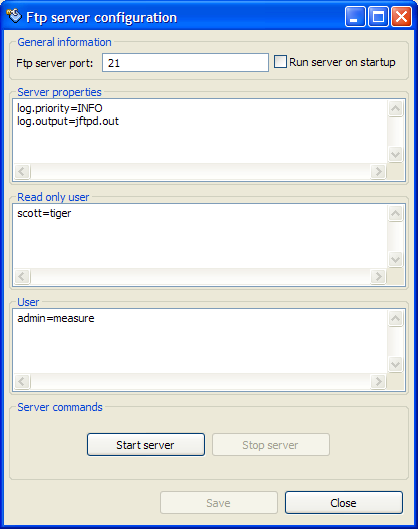
\includegraphics[width=0.6\linewidth]{figures/gui/03.png}
\end{center}
\caption{Okno konfiguracji serwera FTP}\label{rys:ftpwindow}
\end{figure}
Pole tekstowe ,,Server properties'' służy do ustawiania specyficznych właściwości serwera.
Wpisuje się tutaj pary klucz--wartość. W chwili obecnej dostępne są dwa klucze:
\begin{itemize}
\item log.prority -- określa priorytet logowanych operacji dla serwera FTP. Dostępne są następujące wartości:
\begin{itemize}
\item NONE -- powoduje wyłączenie logowania,
\item INFO -- loguje wszystkie dostępne informacje,
\item DEBUG -- loguje błędy i informacje przydatne w procesie debugowania,
\item ERROR -- loguje tylko błędy.
\end{itemize}
Informacje te są zapisywane w pliku wskazywanym przez klucz ,,log.output''.
\item log.output -- wskazuje położenie pliku z logami.
\end{itemize}
Serwer ftp jak i cała aplikacja używa do logowania operacji biblioteki Log4J~\cite{Log4J1}.

Pole tekstowe ,,Read only user'' umożliwia podanie użytkowników z prawami tylko do odczytu z serwera FTP.
W polu tym w każdej linii umieszcza się pary klucz--wartość, gdzie klucz odpowiada loginowi użytkownika,
a wartość to hasło. 

Pole tekstowe ,,User'' umożliwia podanie użytkowników z pełnymi prawami do serwera FTP. Tacy użytkownicy
mogą dodawać, modyfikować i usuwać pliki dostępne na serwerze ftp benchmarku.

\section{Server RMI}\label{sect:rmiserver}
Do komunikacji pomiędzy serwerem, a klientami RTE aplikacja wykorzystuje serwer
RMI~\cite{RMI1}. Można go skonfigurować wybierając z menu ,,Configuration'' opcję ,,RMI server''. 
Wybranie tej opcji powoduje wyświetlenie okienka widocznego na rys.~\ref{rys:rmiwindow}.
\begin{figure}[h]
\begin{center}
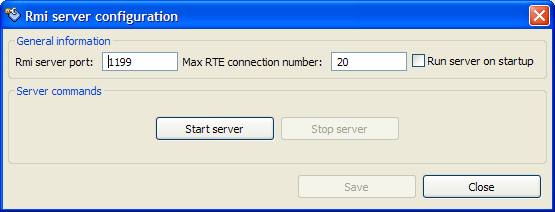
\includegraphics[width=0.70\linewidth]{figures/gui/04.png}
\end{center}
\caption{Okno konfiguracji serwera RMI}\label{rys:rmiwindow}
\end{figure}
Jak widać, w tym miejscu można określić: numer portu na którym ma nasłuchiwać serwer,
maksymalną liczbę klientów RTE, którzy mogą podłączyć się do serwera, czy serwer ma być
uruchamiany wraz z uruchomieniem aplikacji.

\section{Projekt testu}
Aplikacja GUI serwera benchmarku umożliwia tworzenie projektów testów,
które chcemy przeprowadzić. W tym celu należy z menu ,,File'' wybrać opcję ,,Create test...''.
W wyświetlonym kreatorze istnieje możliwość utworzenia pustego projektu, skopiowania modeli
z jednego z istniejących projektów, lub szablonów (zob. rys.~\ref{rys:createproject}).
\begin{figure}[h]
\begin{center}
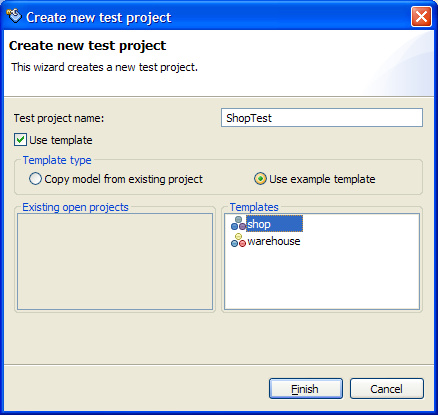
\includegraphics[width=0.5\linewidth]{figures/gui/07.png}
\end{center}
\caption{Kreator projektu testu}\label{rys:createproject}
\end{figure}
Po wybraniu przycisku ,,Finish'' zostanie utworzony projekt testu. Struktura typowego projektu 
została przedstawiona na rys. \ref{rys:testprojectstr}.
\begin{figure}[h]
\begin{center}
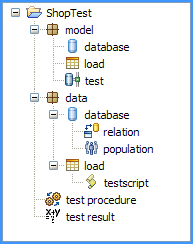
\includegraphics[width=0.3\linewidth]{figures/gui/10.png}
\end{center}
\caption{Struktura projektu testu}\label{rys:testprojectstr}
\end{figure}
Została ona zorganizowana w drzewo dzielące ją na kilka kategorii:
,,model'', ,,data'', ,,test procedure'', ,,test result''. Praca z testem powinna przebiegać
zgodnie z zasadą przechodzenia od liści drzewa usytuowanych najwyżej, do tych usytuowanych najniżej.

Gałąź ,,model'' zawiera modele dostępne dla projektu testu -- są to modele opisane już powyżej, 
a reprezentowane przez liście drzewa: ,,database'', ,,load'' oraz ,,test''.

Gałąź ,,data'' zawiera w sobie wszystkie operacje związane z generowaniem i przygotowywaniem danych niezbędnych
do przeprowadzenia testu. Gałąź ta dzieli się na dwie podgałęzie: ,,database'' -- grupującą operacje
związane z bazą danych, oraz ,,load''-- związaną z generowaniem danych symulujących obciążenie.
W gałęzi ,,database'' dostępne są dwa kreatory: pierwszy do tworzenia bądź usuwania relacji z bazy danych -- ,,relation'',
drugi do generowania populacji -- ,,population''. W gałęzi ,,load'' znajduje się tylko jeden liść -- ,,testscript'', 
reprezentujący kreator tworzenia skryptów testowych. 

Liść ,,test procedure'' reprezentuje kreator przeprowadzania procedury testu.

Liść ,,test result'' zawiera generator raportów i histogramów z wyników przeprowadzonej procedury testu.

\section{Tworzenie modeli}
Aplikacja graficzna serwera benchmarku umożliwia tworzenie modeli bazy danych, obciążenia oraz testu (zob.~rozdz.\ref{rodz:over}). 
Modele te można wpisać posługując się formatem XML, bądź skorzystać z dostępnych formularzy. W załączniku do niniejszej pracy zostały
umieszczone opisy struktury dokumentów xml poszczególnych modeli w postaci XmlSchema~\cite{XmlSchema1}.

\subsection{Model bazy danych}
Model bazy danych można edytować posługując się edytorem dostępnym po wybraniu z
drzewa struktury testu ścieżki ,,model -$>$ database''. W wyniku tej operacji w
głównej części okna aplikacji zostanie wyświetlony edytor modelu bazy danych (zob. rys.~\ref{rys:databaseedytor}).
\begin{figure}[h]
\begin{center}
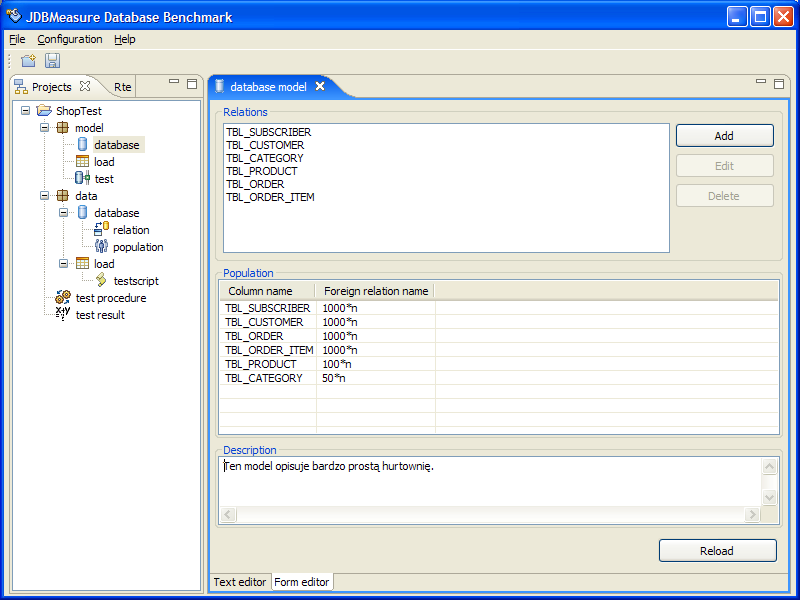
\includegraphics[width=0.9\linewidth]{figures/gui/12.png}
\end{center}
\caption{Edytor modelu bazy danych}\label{rys:databaseedytor}
\end{figure}
W dolnej części edytora znajdują się zakładki umożliwiające przełączanie
pomiędzy edytorem tekstowym, a edytorem opartym o formularze i okna dialogowe.
Edytor tekstowy umożliwia bezpośrednią modyfikację dokumentu xml reprezentującego model bazy danych.
,,Form edytor'' dostarcza natomiast metody modyfikacji dokumentu przy pomocy okien i formularzy.

Sekcja ,,Relations'' edytora umożliwia modyfikację relacji modelu bazy danych. Dostępna jest tutaj lista zdefiniowanych 
relacji. Każdą relację można wyedytować, czy usunąć służą do tego odpowiednio przyciski ,,Edit'' oraz ,,Delete''.
Można również dodać nową relację -- w tym celu należy posłużyć się przyciskiem ,,Add''. 

Sekcja ,,Population'' służy do określenia dla każdej zdefiniowanej relacji, liczby generowanych, w procesie
tworzenia populacji -- rekordów. Można tutaj podać wartość stałą, lub wyrażenie względem parametru skalującego n.

Ostatnią sekcją jest tutaj ,,Description'' -- umożliwia ona podanie opisu tekstowego tworzonego modelu bazy danych.

\subsection{Model obciążenia}
Model obciążenia można edytować posługując się edytorem dostępnym po wybraniu z
drzewa struktury testu ścieżki ,,model -$>$ load''. W wyniku tej operacji w
głównej części okna aplikacji zostanie wyświetlony edytor modelu obciążenia (zob. rys.~\ref{rys:loadedytor}).
\begin{figure}[h]
\begin{center}
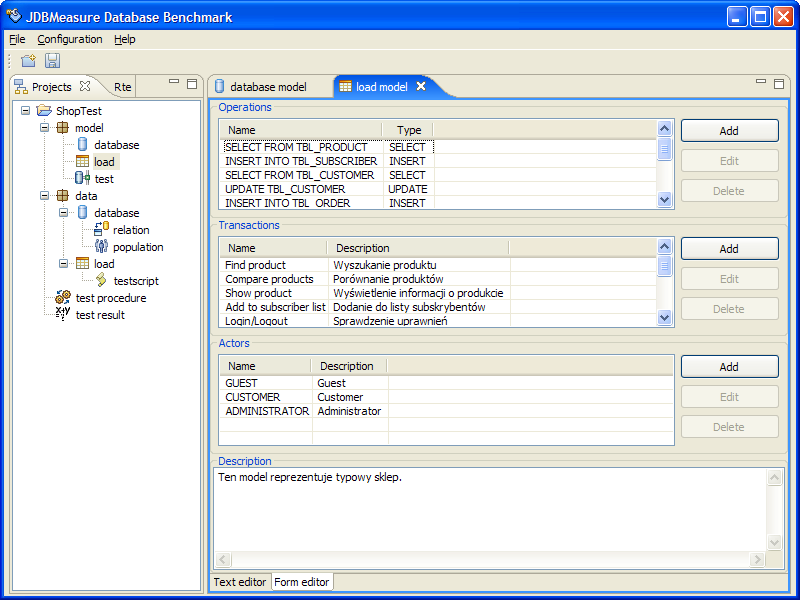
\includegraphics[width=0.9\linewidth]{figures/gui/14.png}
\end{center}
\caption{Edytor modelu obciążenia}\label{rys:loadedytor}
\end{figure}
W dolnej części edytora znajdują się zakładki umożliwiające przełączanie
pomiędzy edytorem tekstowym, a edytorem opartym o formularze i okna dialogowe.
Edytor tekstowy umożliwia bezpośrednią modyfikację dokumentu xml reprezentującego model obciążenia.
,,Form edytor'' dostarcza natomiast metody modyfikacji dokumentu przy pomocy okien i formularzy.

Sekcja ,,Operations'' służy do dodawania i modyfikacji operacji zdefiniowanych w modelu obciążenia.
W tym celu należy posłużyć się przyciskami ,,Add'', ,,Edit'' oraz ,,Delete''.
W sekcji tej znajduje się także lista istniejących w modelu operacji.

Sekcja ,,Transaction'' zawiera listę zdefiniowanych w modelu transakcji. Lista ta może być modyfikowana
za pomocą znajdujących się na prawo od niej przycisków  ,,Add'', ,,Edit'' oraz ,,Delete''.

Sekcja ,,Actors'' jest przeznaczona do edycji listy zdefiniowanych w modelu aktorów. W tym celu należy posłużyć się przyciskami
,,Add'', ,,Edit'' oraz ,,Delete''.

W dolnej części edytora znajduje się sekcja ,,Description'' umożliwiająca wprowadzenie opisu tekstowego dla modelu obciążenia.

\subsection{Model testu}
Model testu można edytować posługując się edytorem dostępnym po wybraniu z
drzewa struktury testu ścieżki ,,model -$>$ test''. W wyniku tej operacji w
głównej części okna aplikacji zostanie wyświetlony edytor modelu test (zob. rys.~\ref{rys:testedytor}).
\begin{figure}[h]
\begin{center}
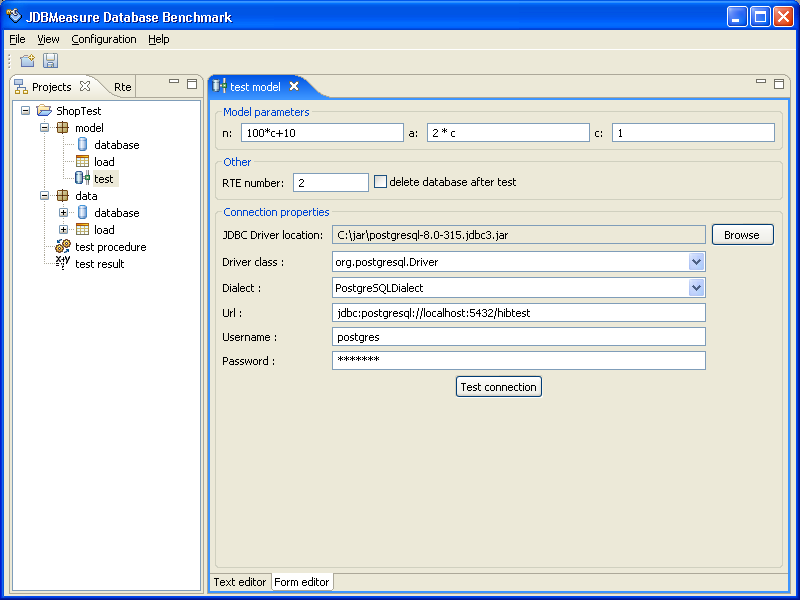
\includegraphics[width=0.9\linewidth]{figures/gui/16.png}
\end{center}
\caption{Edytor modelu testu}\label{rys:testedytor}
\end{figure}
W dolnej części edytora znajdują się zakładki umożliwiające przełączanie
pomiędzy edytorem tekstowym, a edytorem opartym o formularze i okna dialogowe.
Edytor tekstowy umożliwia bezpośrednią modyfikację dokumentu xml reprezentującego model testu.
,,Form edytor'' dostarcza natomiast metody modyfikacji dokumentu przy pomocy okien i formularzy.
Edytor ten umożliwia zdefiniowanie modelu testu, ułatwia przy tym określenie sterownika JDBC,
a także umożliwia przetestowanie połączenia z bazą danych.

Sekcja ,,Model parameters'' umożliwia określenie wartości parametrów skalujących:
\begin{itemize}
\item ,,n'' -- jest parametrem skalującym wykorzystywanym w modelu bazy danych, do określenia liczby 
generowanych rekordów dla poszczególnych relacji, w procesie generowania populacji,
\item ,,a'' -- jest parametrem skalującym wykorzystywanym w modelu obciążenia, do definiowania minimalnej 
i~maksymalnej liczby aktorów danego typu,
\item ,,c'' -- jest parametrem służącym do powiązania parametrów ,,n'' i ,,a''.
\end{itemize}
Więcej informacji na temat parametrów skalujących znajduje się w podpunkcie~\ref{sect:testmodel}.

Sekcja ,,Other'' zawiera opcje konfiguracyjne modelu testu nie sklasyfikowane nigdzie indziej. Można
tutaj określić liczbę RTE biorących udział w teście, jak i to czy baza danych ma być usunięta po zakończeniu testu.
Warto w tym miejscu zauważyć, iż zwiększenie liczby RTE nie powoduje zwiększenia obciążenia, gdyż obciążenie zdefiniowane
w modelu obciążenia jest dzielone na wszystkie RTE biorące udział w teście. Tak więc zwiększając liczbę RTE zmniejszamy
porcję generowanego obciążenia przez pojedyncze RTE. Dla bazy danych rośnie natomiast liczba potencjalnych konfliktów
przydziału zasobów, wynikających z wielodostępu.

Sekcja ,,Connection properties'' zawiera właściwości połączenia do bazy danych. ,,JDBC Driver location'' służy do wskazania
sterownika JDBC, który ma zostać użyty w teście. W celu zmiany wartości tej właściwości należy wybrać przycisk ,,Browse''.
Po dokonaniu tej operacji zostanie wyświetlone okienko, umożliwiające wskazanie lokalizacji sterownika. Warto tutaj zauważyć,
iż sterowniki nie wchodzą bezpośrednio w skład benchmarku. Należy zatem pobrać niezbędny sterownik JDBC ze strony producenta 
testowanego SZBD lub z innej lokalizacji. Lista rozwijana ,,Driver class'' służy do wyboru jednej ze znalezionych w bibliotece 
sterownika JDBC klasy sterownika. Lista rozwijana ,,Dialect'' umożliwia wybór dialektu testowanej bazy danych. To od wybranego dialektu
zależy sposób generowania skryptów tworzących i usuwających bazę danych, a także sposób obsługi obiektów LOB. Kolejną właściwością
jest tutaj ,,Url''. Jest to łańcuch znakowy umożliwiający sterownikowi JDBC zlokalizowanie bazy danych. Dokładna struktura
tego łańcucha zależy od typu bazy danych i od danego sterownika. Dlatego bliższych informacji na ten temat należy szukać w dokumentacji 
używanego sterownika JDBC. Ostatnimi parametrami sekcji są ,,Username'' i ,,Password''. Służą one do uwierzytelniania i 
autoryzacji dostępu do bazy danych.

\begin{figure}[!h]
\begin{center}
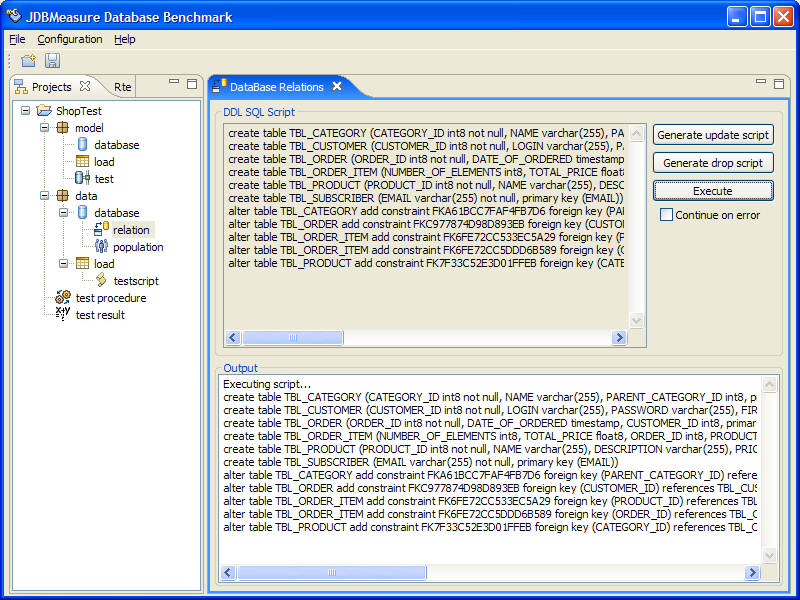
\includegraphics[width=0.9\linewidth]{figures/gui/18.png}
\end{center}
\caption{Edytor relacji}\label{rys:relationsedytor}
\end{figure}

\section{Generowanie danych}
Kolejnym etapem pracy z benchmarkiem -- po zdefiniowaniu modeli, jest przygotowanie
danych potrzebnych w procedurze testu. Dane te można przygotować przy pomocy
edytorów/kreatorów dostępnych w gałęzi data drzewa struktury projektu testu.
\subsection{Tworzenie/usuwanie relacji}
W celu stworzenia na podstawie modelu bazy danych relacji w fizycznej bazie danych
należy wybrać liść ,,data-$>$database-$>$relation''. W wyniku tej operacji zostanie
wyświetlony edytor relacji (zob. rys.~\ref{rys:relationsedytor}).
Edytor ten umożliwia wygenerowanie, dla konkretnego określonego w modelu testu -- DBMS,
skryptów języka SQL, tworzących lub usuwających relacje z bazy danych, a także ich wykonanie.

W celu stworzenia struktury bazy danych należy posłużyć się przyciskiem ,,Generate update script'',
a następnie ,,Execute''. Przycisk ,,Generate update script'' służy do wygenerowania na 
podstawie modelu bazy danych i~modelu testu skryptów tworzących relacje i~powiązania między nimi.

Aby usunąć istniejące relacje, należy wygenerować przyciskiem ,,Generate drop script''
skrypt usuwający relacje, a następnie wykonać go przyciskiem ,,Execute''.

W sekcji ,,DDL SQL Script'' znajduje się pole tekstowe z podglądem wygenerowanych skryptów,
sekcja ,,Output'' zawiera pole tekstowe z komunikatami dotyczącymi wykonywania skryptów.

\subsection{Tworzenie populacji}
Kolejnym edytorem jest tzw. ,,Generator populacji''(zob. rys.~\ref{rys:populationgenerator}). 
Generator ten służy do wygenerowania na podstawie modelu bazy danych, modelu obciążenia 
oraz modelu testu, populacji dla bazy danych. Generator dostępny jest poprzez 
zaznaczenie w drzewie opcji ,,data-$>$database-$>$population''.
\begin{figure}[h]
\begin{center}
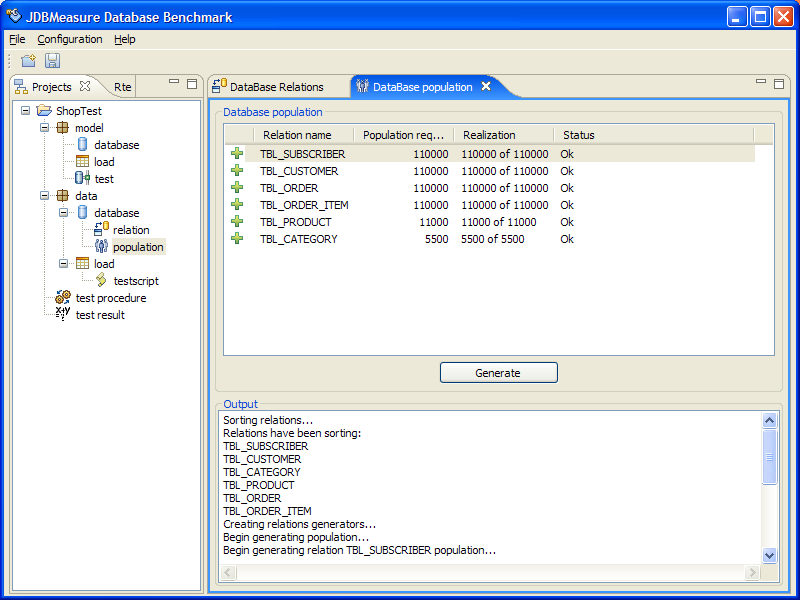
\includegraphics[width=0.9\linewidth]{figures/gui/21.png}
\end{center}
\caption{Generator populacji}\label{rys:populationgenerator}
\end{figure}

\subsection{Przygotowanie skryptów testowych}
Ostatnim narzędziem służącym do przygotowania danych, jest kreator skryptów testowych (zob. rys.~\ref{rys:testscriptscreator}).
W celu wyświetlenia kreatora należy zaznaczyć w drzewie struktury opcję ,,data-$>$load-$>$testscript''
Kreator ten na podstawie wszystkich 3 modeli i zawartości populacji bazy danych
przygotowuje zestaw skryptów testowych. Liczba wygenerowanych skryptów jest zgodna z liczbą RTE wymaganych
do przeprowadzenia procedury testu. Warto zauważyć, że operacja ta nie wymaga 
podłączania RTE do serwera, dzięki temu następuje minimalizacja czasu, w którym 
należy zestawić infrastrukturę testu -- tzn. podłączyć wszystkie wymagane RTE do serwera.
\begin{figure}[h]
\begin{center}
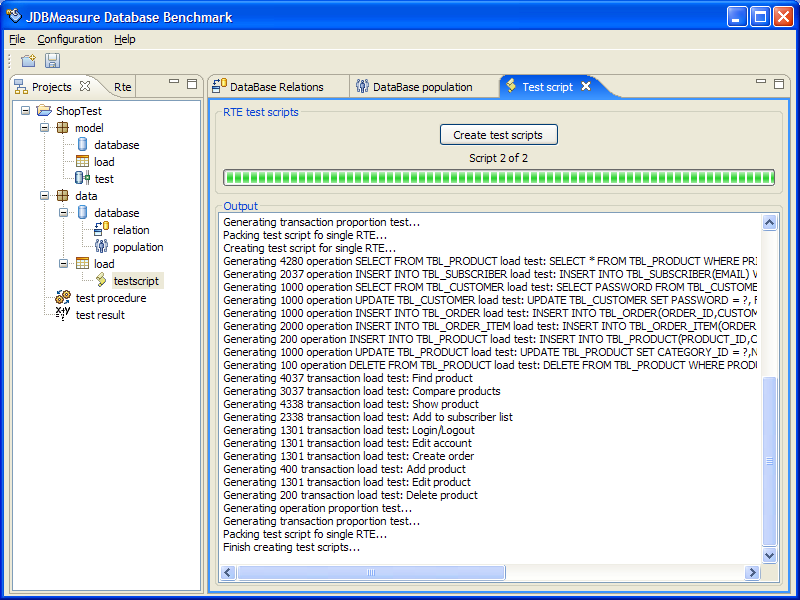
\includegraphics[width=0.9\linewidth]{figures/gui/23.png}
\end{center}
\caption{Kreator skryptów testowych}\label{rys:testscriptscreator}
\end{figure}

\begin{figure}[!h]
\begin{center}
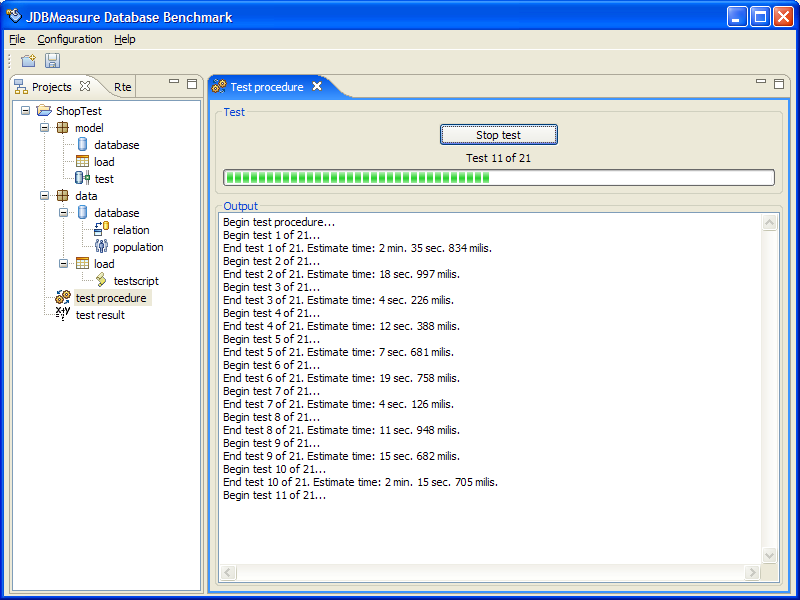
\includegraphics[width=0.9\linewidth]{figures/gui/28.png}
\end{center}
\caption{Przeprowadzanie procedury testu}\label{rys:testprocedure}
\end{figure}

\section{Przeprowadzanie procedury testu}
Przed rozpoczęciem procedury testu należy uruchomić serwer RMI (zob.~\ref{sect:rmiserver}),
a także uruchomić wymaganą liczbę klientów RTE, tak jak omówiono to w rozdz.~\ref{sect:infra}. 
Z przeprowadzaniem procedury testu związany jest widok dostępny po wybraniu z drzewa struktury 
opcji ,,test procedure'' (zob.~rys.~\ref{rys:testprocedure}).

\section{Analiza wyników}
Jeżeli procedura testu zakończyła się powodzeniem można przystąpić do analizy wyników
testów. W tym celu należy przejść do ,,edytora wyników testu'' dostępnego po wybraniu z
drzewa struktury opcji ,,test result''. W edytorze testu dostępne są trzy zakładki
omówione poniżej.

\subsection{Raport tekstowy}
Raport tekstowy jest elementem pierwszej zakładki ,,edytora wyników testu''(zob. rys.~\ref{rys:textraport}). Raport ten został
omówiony szczegółowo w punkcie \ref{sect:textraport}. W załączniku dostępny
jest wydruk przykładowego raportu.
\begin{figure}[h]
\begin{center}
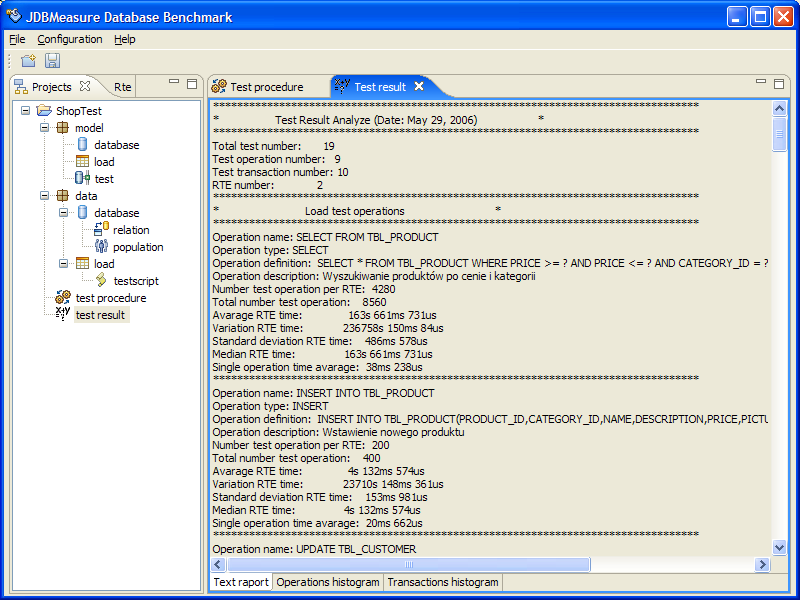
\includegraphics[width=0.9\linewidth]{figures/gui/30.png}
\end{center}
\caption{Raport tekstowy}\label{rys:textraport}
\end{figure}

\subsection{Wykresy}
Pozostałe dwie zakładki ,,edytora wyników testu'' stanowią wykresy histogramów
dla operacji(zob. rys.~\ref{rys:histoper}) i transakcji(zob. rys.~\ref{rys:histtrans}).
Histogramy te obrazują rozkład odpowiedzi dla operacji/transakcji. Możliwe jest określenie
liczby przedziałów histogramów. Wykresy udostępniają funkcje umożliwiające skalowanie,
a także wydruk. Podczas tworzenia histogramów wykorzystano darmową bibliotekę JFreeChart~\cite{JFreeChart1}.
W górnej części zakładki ,,Operations histogram'' znajduje się rozwijana lista, umożliwiająca wybranie interesującej operacji,
na prawo od niej w polu ,,Partitions number'' można określić liczbę przedziałów dla histogramu. Odświeżenie wykresu 
następuje po wyborze przycisku ,,Refresh''. Klikając prawym przyciskiem myszy na obszarze wykresu uzyskuje się dostęp
do menu kontekstowego z opcjami konfiguracyjnymi, a także możliwością wydrukowania wykresu. Przytrzymanie lewego przycisku myszy 
na obszarze wykresu, a następnie przeciągnięcie kursora i puszczenie przycisku, powoduje powiększenie prostokątnego obszaru,
o przekątnej pomiędzy punktem przytrzymania, a puszczenia. Podobną funkcjonalność posiada zakładka ,,Transactions histogram''. 

\begin{figure}[!h]
\begin{center}
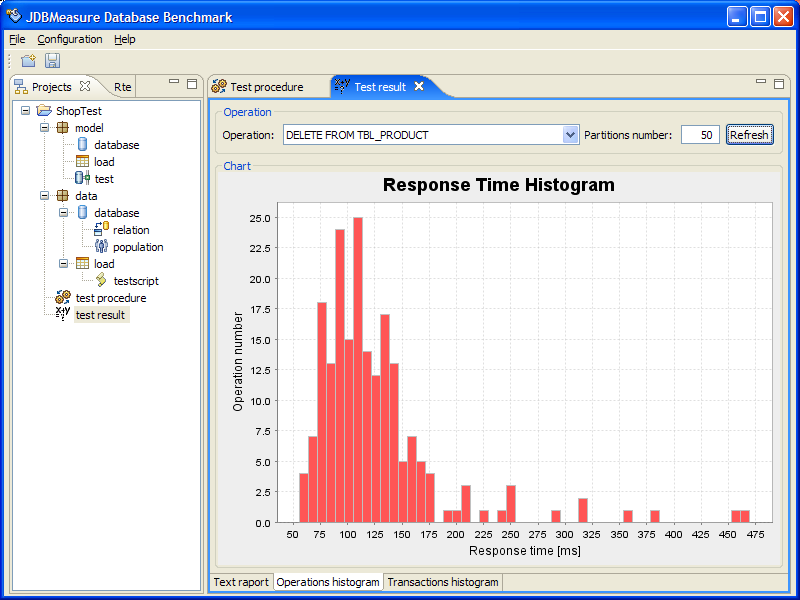
\includegraphics[width=0.9\linewidth]{figures/gui/31.png}
\end{center}
\caption{Histogram czasu wykonania operacji}\label{rys:histoper}
\end{figure}

\begin{figure}[!h]
\begin{center}
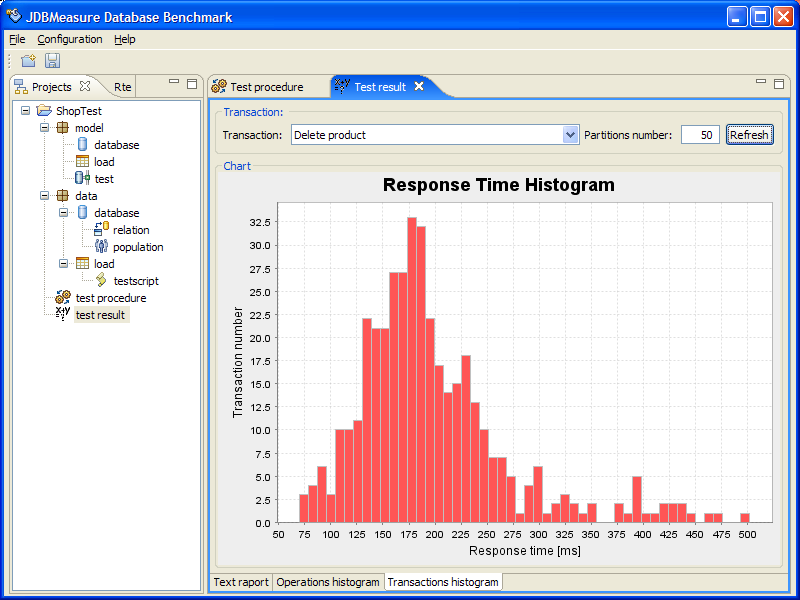
\includegraphics[width=0.9\linewidth]{figures/gui/32.png}
\end{center}
\caption{Histogram czasu wykonania transakcji}\label{rys:histtrans}
\end{figure}

\section{Podsumowanie}
Interfejs graficzny aplikacji serwera benchmarku umożliwia wykonanie
wszystkich niezbędnych operacji, z jakimi użytkownik może mieć do czynienia,
podczas pracy z benchmarkiem. Udostępnia mechanizmy umożliwiające kopiowanie modeli z istniejących projektów,
jak i użycie szablonów sklepu lub hurtowni. Ponadto dzięki poczynionym staraniom automatyzuje
szereg żmudnych i czasochłonnych działań. Dzięki zastosowanym technologiom -- Eclipse RCP \cite{RCP1}, możliwe jest łatwe
rozszerzanie jej o nowe funkcjonalności takie jak:
\begin{enumerate}
\item Edytor XML z podpowiadaniem składni, ułatwiający edycję modeli.
\item Edytory graficzne oparte o biblioteki GEF~\cite{GEF1}, EMF~\cite{EMF1} lub GMF~\cite{GMF1}. Takie edytory 
umożliwiły by wizualne tworzenie modeli tak jak zostało to zilustrowane na rys.~\ref{rys:database-model} 
oraz rys.~\ref{rys:load-model}.
\end{enumerate}


\chapter{Testy benchmarku}\label{chap:test_bench}

Omawiany w tej pracy benchmark został poddany szeregowi testów, począwszy od testów jednostkowych
pojedynczych klas i modułów, przez testy współpracy z różnymi DBMS, po testy mające na celu przyjrzenie się
uzyskiwanym wynikom przy różnej liczbie RTE. 

Testy jednostkowe zostały oparte o bibliotekę JUnit~\cite{JUnit1}. Ich pomyślne przejście było niezbędne do 
przeprowadzenia pozostałych testów. Testy te skupiały się głównie na sprawdzeniu poprawności działania pojedynczych 
klas czy modułów.

Drugą grupę stanowiły testy polegające na sprawdzeniu czy benchmark poprawnie przechodzi przez wszystkie kroki
procedury testowej dla dwóch wybranych modeli -- sklepu i hurtowni danych, oraz dla trzech różnych DBMS -- MySQL 5.0~\cite{MySql1},
PostgreSQL 8.1~\cite{PostgreSql1} i Oracle 10g~\cite{Oracle1}.

Trzecią grupę stanowiły testy wybranego DBMS przy stałym obciążeniu i zmiennej liczbie RTE. Niniejszy rozdział omawia właśnie
testy tego rodzaju.

\section{Środowisko testowe}
Omawiane w tym rozdziale testy zostały przeprowadzone na trzech komputerach A, B i C. Komputery te zostały połączone 
bezpośrednio siecią Fast Ethernet 100Mb/s. Konfiguracja komputerów została przedstawiona w tabelach \ref{tab:kompa},
\ref{tab:kompb} oraz \ref{tab:kompc}. 

\begin{table}[h]
\caption{Konfiguracja komputera A}\label{tab:kompa}
\begin{center}
\begin{tabular}{|l|l|}
\hline
Procesor&AMD Athlon 1.4 GHz\\
\hline
Pamięć RAM&512MB DDRAM\\
\hline
Dysk twardy&40GB\\
\hline
System operacyjny&Windows XP Professional SP2\\
\hline
\end{tabular}
\end{center}
\end{table}

\begin{table}[h]
\caption{Konfiguracja komputera B}\label{tab:kompb}
\begin{center}
\begin{tabular}{|l|l|}
\hline
Procesor&Pentium 2 350MHz\\
\hline
Pamięć RAM&320MB SDRAM\\
\hline
Dysk twardy&40GB Seagate Baracuda\\
\hline
System operacyjny&Windows XP Professional\\
\hline
\end{tabular}
\end{center}
\end{table}

\begin{table}[h]
\caption{Konfiguracja komputera C}\label{tab:kompc}
\begin{center}
\begin{tabular}{|l|l|}
\hline
Procesor&Pentium 3 700MHz\\
\hline
Pamięć RAM&128MB SDRAM\\
\hline
Dysk twardy&10GB\\
\hline
System operacyjny&Windows XP Professional\\
\hline
\end{tabular}
\end{center}
\end{table}

W testach wykorzystano bazę danych MySQL 5.1 -- została ona uruchomiona na komputerze A.
Przed każdym testem baza danych była czyszczona, tworzona była nowa struktura relacji i generowana nowa populacja.
W testach wykorzystano model sklepu dołączony standardowo do benchmarku. Liczba RTE na poszczególnych komputerach 
została podana w tabeli \ref{tab:rterozkl}.

\begin{table}[h]
\caption{Rozkład RTE}\label{tab:rterozkl}
\begin{center}
\begin{tabular}{|r|r|r|r|}
\hline
Całkowita liczba RTE&Na komp. A&Na komp. B&Na komp. C\\
\hline
2&0&1&1\\
\hline
3&0&2&1\\
\hline
4&0&2&2\\
\hline
5&0&3&2\\
\hline
8&1&4&3\\
\hline
\end{tabular}
\end{center}
\end{table}

\section{Wyniki}
Analizie poddano cztery wybrane operacje:
\begin{itemize}
\item selekcję produktu,
\item wstawienie rekordu do tabeli subskrypcji,
\item wstawienie rekordu do tabeli elementów zamówienia, 
\item usunięcie rekordu z tabeli produktów.
\end{itemize}

Na wykresach rys.~\ref{rys:chart_load} oraz rys.~\ref{rys:chart_prop} przedstawiono zbiorczo
wyniki testów obciążeniowych i proprocjonalnościowych. Tabele z wynikami testów zostały zamieszczone w załączniku.
Wszystkie czasy zostały podane w mikrosekundach.

\section{Wnioski}
Z zebranych danych można wysnuć następujące wnioski:
\begin{enumerate}
\item Czas wykonania danego testu obciążeniowego na pojedynczym RTE, przy wzrastającej liczbie RTE 
i tych samych parametrach skalujących spada. Przy czym wartość tego spadku zależy od typu operacji -- im
operacja jest bardziej złożona tym spadek jest mniejszy. Przez złożoność operacji należy rozumieć wpływ
na szybkość jej przeprowadzenia innych operacji aktualnie znajdujących się w systemie. Wpływ ten będzie wynikał
w głównej mierze z konieczności zapewnienia atomowości operacji. Spadek czasu wykonania testu wynika z mniejszej 
liczby operacji/transakcji przypadających na pojedynczy RTE. 

Reguła ta w przeprowadzonych testach nie sprawdziła się dla testu obciążeniowego selekcji produktu, dla tej operacji
czas ten wzrastał. Istnieje podejrzenie, iż przyczyną tego mogły być zbyt małe bufory pamięci przeznaczone na operacje
łączenia wyników zapytań. W tej operacji zbiór wynikowy mógł być duży, w połączeniu z wzrastającą wraz z liczbą RTE 
liczbą równoległych żądań, bufory te mogły ulec przeciążeniu.
\item Średni czas wykonania pojedynczej operacji rośnie.
\item Odchylenie standardowe względem średniego czasu wykonania pojedynczej operacji rośnie
\item Najmniej stabilne wyniki uzyskano dla operacji usunięcia produktu, na fakt ten z pewnością wpłynęła konieczność dokonywania
przez DBMS kaskadowego usuwania rekordów z relacji dotyczących zamówień.
\end{enumerate}

\begin{figure}[p]
\begin{center}
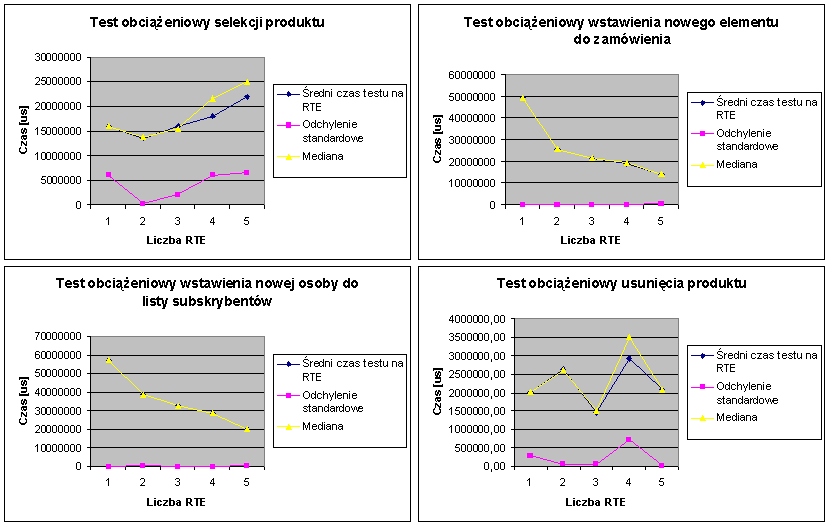
\includegraphics[width=1.1\linewidth]{figures/chart_load.png}
\end{center}
\caption{Wykresy dla testów obciążeniowych}\label{rys:chart_load}
\end{figure}

\begin{figure}[p]
\begin{center}
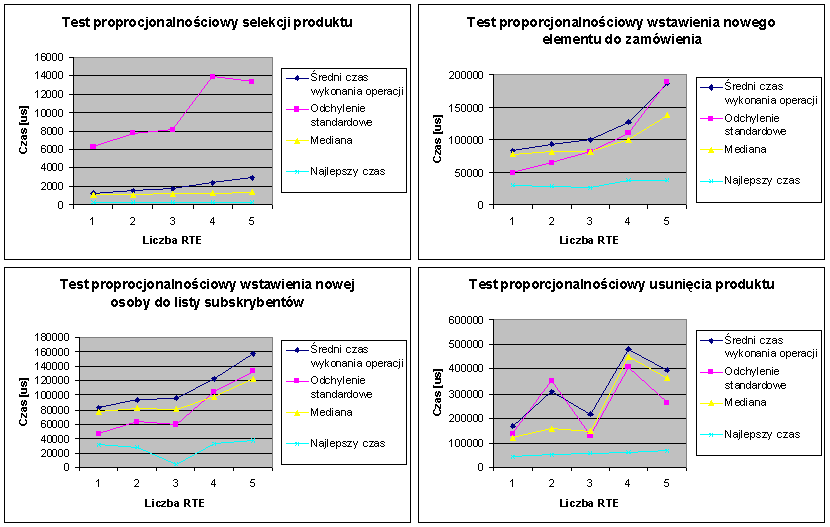
\includegraphics[width=1.1\linewidth]{figures/chart_prop.png}
\end{center}
\caption{Wykresy dla testów proporcjonalnościowych}\label{rys:chart_prop}
\end{figure}



\chapter{Wnioski i podsumowanie prac}
Rozdział ten stanowi krótkie podsumowanie prac związanych z budową benchmarku,
jak i odpowiedź na postawione na początku pracy pytania i cele. Wskazuje także kierunki dalszego rozwoju.

\section{Wyniki i wnioski z prac}
Podstawowym celem niniejszej pracy było stworzenie benchmarku, który umożliwiałby mierzenie
wydajności SZBD. Autorowi nie chodziło jednak o stworzenie typowego benchmarku
wraz ze związanymi z nim ograniczeniami min.:
\begin{itemize}
\item jednym niemodyfikowalnym modelem,
\item występowaniem często jako specyfikacja, którą trzeba dla każdego DBMS niezależnie implementować,
\item testowaniem jednego konkretnego DBMS.
\end{itemize}
Głównym celem było przezwyciężenie powyższych ograniczeń i stworzenie narzędzia,
bardziej uniwersalnego, posiadającego szerszą gamę zastosowań.
Co zatem uzyskano? Czy stworzony benchmark spełnia powyższe kryteria?
W stworzonym benchmarku definicja testu, procedury testowej, składa się z trzech modeli.
Podział taki, ułatwia definiowanie testu, każdy model ma bowiem ściśle określone przeznaczenie, 
razem zaś stanowią pełną definicję, uwzględniającą wszystkie aspekty rzeczywistego 
systemu opartego o współpracę z DBMS. Takie podejście ułatwia definiowanie testu niezależnie od DBMS. Zmiana DBMS 
sprowadza się do zmiany dialektu i parametrów połączenia w modelu testu. Koncepcja 
taka zapewnia również łatwą, wielokryterialną skalowalność. Sama procedura testu jest niezależna 
od jednego konkretnego modelu bazy danych, czy modelu obciążenia. Wykorzystanie 
języka Java i sterowników JDBC umożliwia testowanie różnych DBMS, jak i uruchamianie
benchmarku na różnych systemach operacyjnych.

Zbudowany benchmark charakteryzują najpełniej następujące cechy:
\begin{itemize}
\item niezależność modelu od konkretnego DBMS,
\item niezależność procedury testu od konkretnego modelu,
\item niezależność mechanizmów analizy wyników od konkretnego modelu,
\item możliwość testowania różnych DBMS (Oracle, PostgreSQL, MySQL),
\item możliwość testowania różnych baz danych,
\item możliwość definiowania własnych modeli baz danych i obciążenia,
\item możliwość analizy modelu bazy danych rzeczywistego systemu i analizy modelu obciążenia,
\item możliwość porównywania wydajności różnych sterowników JDBC.
\end{itemize}

\section{Propozycje dalszego rozwoju}

Budując dowolny system informatyczny w pierwszej kolejności należy wyrzec się 
przeświadczenia o własnej nieomylności, a także przekonania, że stworzone rozwiązanie
będzie rozwiązaniem idealnym, nie wymagającym w przyszłości zmian. 
Użytkownicy są bowiem najlepszym weryfikatorem stworzonego rozwiązania i podjętych decyzji projektowych.
To bowiem zbudowane rozwiązanie jest dla nich i nigdy na odwrót.
W świecie inżynierii oprogramowania istnieje powiedzenie, iż ,,system nie jest dobry
przed wersją trzecią''. Trudno nie zgodzić się z powyższymi stwierdzeniami. Również
stworzony benchmark, jest pewnym kompromisem. 

Autor zatem, świadomy opisanych powyżej problemów dołożył wszelkich starań by 
zbudowane rozwiązanie było łatwe w rozbudowie czy modyfikacji.

Jeżeli benchmark znajdzie zastosowanie to z pewnością w przyszłości będzie istniała konieczność
wprowadzania w nim modyfikacji. Już na etapie prac zauważono, iż dla modeli
bazy danych i obciążenia najlepszym rozwiązaniem było by stworzenie edytorów graficznych.
Ze względu jednak na inny priorytet zadań i celów pracy, stworzenie takich edytorów 
zostało wyłączone z niniejszej wersji benchmarku. Nie mniej jednak postanowiono
wykorzystać rozwiązania ułatwiające zbudowanie takich edytorów w przyszłości.
W procesie budowy aplikacji graficznej serwera benchmarku użyto zatem środowiska
Eclipse RCP~\cite{RCP1} w wersji 3.2.

Benchmark można by również rozszerzyć o testy w oparciu o scenariusze. Scenariusz określa 
z ustalonym prawdopodobieństwem kolejność wykonywania operacji/transakcji po sobie. Umożliwia zatem
stworzenie testów jeszcze bardziej zbliżonych do rzeczywistości.




% bibliography starts here.
\bibliographystyle{plain}%plalpha
{\small\bibliography{bibliography}}

% all appendices and extra material come at the end.
\backmatter%
\chapter{Załączniki}

\section{Definicje XMLSchema dla modeli}
\subsection{Model bazy danych}
\begin{Verbatim}
<?xml version="1.0" encoding="UTF-8"?>
<xsd:schema xmlns:xsd="http://www.w3.org/2001/XMLSchema"
	xmlns:tns="http://www.jdbmeasure.org/database-model"
	targetNamespace="http://www.jdbmeasure.org/database-model"
	xmlns="http://www.jdbmeasure.org/database-model"
	elementFormDefault="qualified">
	<xsd:complexType name="tcolumn">
		<xsd:attribute name="name" type="xsd:string" use="required" />
		<xsd:attribute name="type" type="xsd:string" use="required" />
		<xsd:attribute name="is_nullable" type="xsd:boolean" />
		<xsd:attribute name="is_id" type="xsd:boolean" />
		<xsd:attribute name="min_value" type="xsd:string" />
		<xsd:attribute name="max_value" type="xsd:string" />
		<xsd:attribute name="is_lob" type="xsd:boolean" />
		<xsd:attribute name="is_unique" type="xsd:boolean" />
		<xsd:attribute name="unique_group_id" type="xsd:string" />
	</xsd:complexType>
	<xsd:complexType name="treference">
		<xsd:attribute name="column_name" 
			type="xsd:string" use="required" />
		<xsd:attribute name="relation_name" 
			type="xsd:string" use="required" />
		<xsd:attribute name="relation_column_name" 
			type="xsd:string" use="required" />
	</xsd:complexType>
	<xsd:complexType name="tcolumns">
		<xsd:sequence minOccurs="0" maxOccurs="unbounded">
			<xsd:element name="column" type="tns:tcolumn" />
		</xsd:sequence>
	</xsd:complexType>
	<xsd:complexType name="treferences">
		<xsd:sequence minOccurs="0" maxOccurs="unbounded">
			<xsd:element name="reference" type="tns:treference" />
		</xsd:sequence>
	</xsd:complexType>
	<xsd:complexType name="trelation">
		<xsd:sequence minOccurs="0">
			<xsd:element name="columns" type="tns:tcolumns" />
			<xsd:element name="references" type="tns:treferences" minOccurs="0" />
		</xsd:sequence>
		<xsd:attribute name="name" type="xsd:string" use="required" />
	</xsd:complexType>
	<xsd:complexType name="trelations">
		<xsd:sequence minOccurs="0" maxOccurs="unbounded">
			<xsd:element name="relation" type="tns:trelation" />
		</xsd:sequence>
	</xsd:complexType>
	<xsd:complexType name="trelation-population">
		<xsd:attribute name="relation_name" type="xsd:string" use="required" />
		<xsd:attribute name="expression" type="xsd:string" use="required" />
	</xsd:complexType>
	<xsd:complexType name="tpopulation">
		<xsd:sequence minOccurs="0" maxOccurs="unbounded">
			<xsd:element name="relation-population" 
				type="tns:trelation-population" />
		</xsd:sequence>
	</xsd:complexType>
	<xsd:complexType name="tdatabase-model">
		<xsd:sequence minOccurs="0">
			<xsd:element name="relations" type="tns:trelations" />
			<xsd:element name="population" type="tns:tpopulation" />
			<xsd:element name="model-description" type="xsd:string" />
		</xsd:sequence>
	</xsd:complexType>
	<xsd:element name="database-model" type="tns:tdatabase-model" />
</xsd:schema>
\end{Verbatim}

\subsection{Model obciążenia}
\begin{Verbatim}
<?xml version="1.0" encoding="UTF-8"?>
<xsd:schema xmlns="http://www.jdbmeasure.org/load-model"
	xmlns:tns="http://www.jdbmeasure.org/load-model"
	xmlns:xsd="http://www.w3.org/2001/XMLSchema"
	elementFormDefault="qualified"
	targetNamespace="http://www.jdbmeasure.org/load-model">
	<xsd:complexType name="tparameter">
		<xsd:attribute name="number" type="xsd:double" use="required" />
		<xsd:attribute name="type" type="xsd:string" use="required" />
		<xsd:attribute name="is_nullable" type="xsd:boolean" />
		<xsd:attribute name="is_id" type="xsd:boolean" />
		<xsd:attribute name="min_value" type="xsd:string" />
		<xsd:attribute name="max_value" type="xsd:string" />
		<xsd:attribute name="is_lob" type="xsd:boolean" />
		<xsd:attribute name="is_unique" type="xsd:boolean" />
		<xsd:attribute name="unique_group_id" type="xsd:string" />
		<xsd:attribute name="ref_relation_name" type="xsd:string" />
		<xsd:attribute name="ref_relation_column_name" type="xsd:string" />
	</xsd:complexType>
	<xsd:complexType name="tparameters">
		<xsd:sequence minOccurs="0" maxOccurs="unbounded">
			<xsd:element name="parameter" type="tns:tparameter" />
		</xsd:sequence>
	</xsd:complexType>
	<xsd:complexType name="toperation">
		<xsd:sequence minOccurs="1" maxOccurs="unbounded">
			<xsd:element name="definition" type="xsd:string" />
			<xsd:element name="parameters" type="tns:tparameters" />
			<xsd:element name="operation-description" type="xsd:string" />
		</xsd:sequence>
		<xsd:attribute name="name" type="xsd:string" use="required" />
		<xsd:attribute name="type" type="xsd:string" use="required" />
	</xsd:complexType>
	<xsd:complexType name="toperations">
		<xsd:sequence minOccurs="0" maxOccurs="unbounded">
			<xsd:element name="operation" type="tns:toperation" />
		</xsd:sequence>
	</xsd:complexType>
	<xsd:complexType name="ttransaction-operation">
		<xsd:attribute name="operation_name" type="xsd:string" 
			use="required" />
		<xsd:attribute name="number" type="xsd:integer" />
	</xsd:complexType>
	<xsd:complexType name="ttransaction-operations">
		<xsd:sequence minOccurs="0" maxOccurs="unbounded">
			<xsd:element name="transaction-operation" 
				type="tns:ttransaction-operation" />
		</xsd:sequence>
	</xsd:complexType>
	<xsd:complexType name="ttransaction">
		<xsd:sequence minOccurs="0">
			<xsd:element name="transaction-operations" 
				type="tns:ttransaction-operations" />
			<xsd:element name="transaction-description" 
				type="xsd:string" />
		</xsd:sequence>
		<xsd:attribute name="name" type="xsd:string" use="required" />
	</xsd:complexType>
	<xsd:complexType name="ttransactions">
		<xsd:sequence minOccurs="0" maxOccurs="unbounded">
			<xsd:element name="transaction" type="tns:ttransaction" />
		</xsd:sequence>
	</xsd:complexType>
	<xsd:complexType name="tactor-transaction">
		<xsd:attribute name="transaction_name" type="xsd:string" 
			use="required" />
		<xsd:attribute name="avg_call_number" type="xsd:integer" 
			use="required" />
	</xsd:complexType>
	<xsd:complexType name="tactor-transactions">
		<xsd:sequence minOccurs="0" maxOccurs="unbounded">
			<xsd:element name="actor-transaction" 
				type="tns:tactor-transaction" />
		</xsd:sequence>
	</xsd:complexType>
	<xsd:complexType name="tactor">
		<xsd:sequence minOccurs="0">
			<xsd:element name="actor-transactions" 
				type="tns:tactor-transactions" />
			<xsd:element name="actor-description" type="xsd:string" />
		</xsd:sequence>
		<xsd:attribute name="name" type="xsd:string" use="required" />
		<xsd:attribute name="session_length" type="xsd:string" use="required" />
		<xsd:attribute name="min_number" type="xsd:string" use="required" />
		<xsd:attribute name="max_number" type="xsd:string" use="required" />
		<xsd:attribute name="parent" type="xsd:string" />
		<xsd:attribute name="inh_level" type="xsd:double" />
	</xsd:complexType>
	<xsd:complexType name="tactors">
		<xsd:sequence minOccurs="0" maxOccurs="unbounded">
			<xsd:element name="actor" type="tns:tactor" />
		</xsd:sequence>
	</xsd:complexType>
	<xsd:complexType name="tload-model">
		<xsd:sequence minOccurs="0">
			<xsd:element name="operations" type="tns:toperations" />
			<xsd:element name="transactions" type="tns:ttransactions" />
			<xsd:element name="actors" type="tns:tactors" />
			<xsd:element name="description" type="xsd:string" />
		</xsd:sequence>
	</xsd:complexType>
	<xsd:element name="load-model" type="tns:tload-model" />
</xsd:schema>
\end{Verbatim}

\subsection{Model testu}
\begin{Verbatim}
<?xml version="1.0" encoding="UTF-8"?>
<xsd:schema xmlns="http://www.jdbmeasure.org/load-model"
	xmlns:tns="http://www.jdbmeasure.org/load-model"
	xmlns:xsd="http://www.w3.org/2001/XMLSchema"
	elementFormDefault="qualified"
	targetNamespace="http://www.jdbmeasure.org/test-model">
	<xsd:complexType name="tproperty">
		<xsd:attribute name="name" type="xsd:string" />
		<xsd:attribute name="value" type="xsd:string" />
	</xsd:complexType>
	<xsd:complexType name="tjdbc-connection-properties">
		<xsd:sequence minOccurs="6" maxOccurs="6">
			<xsd:element name="property" type="tns:tproperty" />
		</xsd:sequence>
	</xsd:complexType>
	<xsd:complexType name="ttest-model">
		<xsd:sequence minOccurs="1" maxOccurs="1">
			<xsd:element name="jdbc-connection-properties" 
			type="tns:tjdbc-connection-properties" />
		</xsd:sequence>
		<xsd:attribute name="delete_db_after_test" type="xsd:boolean" use="required" />
		<xsd:attribute name="rte_number" type="xsd:integer" use="required" />
		<xsd:attribute name="c" type="xsd:string" use="required" />
		<xsd:attribute name="n" type="xsd:string" use="required" />
		<xsd:attribute name="a" type="xsd:string" use="required" />
	</xsd:complexType>
	<xsd:element name="test-model" type="tns:ttest-model" />
	</xsd:schema>
\end{Verbatim}
	
\section{Przykładowy raport}\label{sect:raportexample}

Poniżej został zamieszczony przykładowy raport w formie tekstowej:\\
\begin{Verbatim}
*********************************************************************************
*                   Test Result Analyze (Date: June 19, 2006)                   *
*********************************************************************************

Total test number:       19
Test operation number:   9
Test transaction number: 10
RTE number:              8

*********************************************************************************
*                             Load test operations                              *
*********************************************************************************
Operation name: DELETE FROM TBL_PRODUCT
Operation type: DELETE
Operation definition:  DELETE FROM TBL_PRODUCT WHERE PRODUCT_ID = ?
Operation description: Usunięcie produktu

Number of test operations per RTE:  2
Total number of test operations:    16

Avarage RTE time:               2s 85ms 61us
Median RTE time:                2s 90ms 362us
Standard deviation RTE time:    24ms 226us

Single operation time avarage:  1s 42ms 530us
*********************************************************************************
Operation name: UPDATE TBL_CUSTOMER
Operation type: UPDATE
Operation definition: UPDATE TBL_CUSTOMER SET PASSWORD = ?, FIRSTNAME = ?, SURNAME = ?, 
                      DATE_OF_BIRTH = ?, SEX = ?, IS_SINGLE = ? WHERE LOGIN = ?
Operation description: Edycja danych osoby

Number of test operations per RTE:  25
Total number of test operations:    200

Avarage RTE time:               9s 380ms 75us
Median RTE time:                9s 271ms 203us
Standard deviation RTE time:    239ms 620us

Single operation time avarage:  375ms 203us
*********************************************************************************
Operation name: INSERT INTO TBL_PRODUCT
Operation type: INSERT
Operation definition: INSERT INTO TBL_PRODUCT(PRODUCT_ID,CATEGORY_ID,NAME,DESCRIPTION,
                      PRICE,PICTURE) VALUES(?,?,?,?,?,?)
Operation description: Wstawienie nowego produktu

Number of test operations per RTE:  5
Total number of test operations:    40

Avarage RTE time:               1s 395ms 474us
Median RTE time:                1s 430ms 633us
Standard deviation RTE time:    136ms 733us

Single operation time avarage:  279ms 94us
*********************************************************************************
Operation name: UPDATE TBL_PRODUCT
Operation type: UPDATE
Operation definition: UPDATE TBL_PRODUCT SET CATEGORY_ID = ?,NAME = ?,
                      DESCRIPTION = ?,PRICE = ?,PICTURE = ? WHERE PRODUCT_ID = ?
Operation description: Edycja produktu

Number of test operations per RTE:  5
Total number of test operations:    40

Avarage RTE time:               1s 113ms 84us
Median RTE time:                1s 132ms 911us
Standard deviation RTE time:    61ms 696us

Single operation time avarage:  222ms 616us
*********************************************************************************
Operation name: INSERT INTO TBL_ORDER
Operation type: INSERT
Operation definition: INSERT INTO TBL_ORDER(ORDER_ID,CUSTOMER_ID,DATE_OF_ORDERED) 
                      VALUES(?,?,?)
Operation description: Wstawienie nowego zamówienia

Number of test operations per RTE:  25
Total number of test operations:    200

Avarage RTE time:               5s 441ms 257us
Median RTE time:                5s 408ms 721us
Standard deviation RTE time:    117ms 831us

Single operation time avarage:  217ms 650us
*********************************************************************************
Operation name: SELECT FROM TBL_CUSTOMER
Operation type: SELECT
Operation definition:  SELECT PASSWORD FROM TBL_CUSTOMER WHERE LOGIN = ?
Operation description: Sprawdzenie uprawnień osoby do systemu

Number of test operations per RTE:  25
Total number of test operations:    200

Avarage RTE time:               3s 931ms 560us
Median RTE time:                3s 996ms 802us
Standard deviation RTE time:    434ms 464us

Single operation time avarage:  157ms 262us
*********************************************************************************
Operation name: INSERT INTO TBL_ORDER_ITEM
Operation type: INSERT
Operation definition: INSERT INTO TBL_ORDER_ITEM(ORDER_ID,PRODUCT_ID,
                      NUMBER_OF_ELEMENTS,TOTAL_PRICE) VALUES(?,?,?,?)
Operation description: Wstawienie nowego elementu do zamówienia

Number of test operations per RTE:  100
Total number of test operations:    800

Avarage RTE time:               13s 868ms 642us
Median RTE time:                13s 870ms 341us
Standard deviation RTE time:    205ms 197us

Single operation time avarage:  138ms 686us
*********************************************************************************
Operation name: INSERT INTO TBL_SUBSCRIBER
Operation type: INSERT
Operation definition:  INSERT INTO TBL_SUBSCRIBER(EMAIL) VALUES(?)
Operation description: Dodanie osoby do listy subskrybentów

Number of test operations per RTE:  147
Total number of test operations:    1176

Avarage RTE time:               19s 945ms 149us
Median RTE time:                19s 982ms 314us
Standard deviation RTE time:    239ms 890us

Single operation time avarage:  135ms 681us
*********************************************************************************
Operation name: SELECT FROM TBL_PRODUCT
Operation type: SELECT
Operation definition: SELECT * FROM TBL_PRODUCT WHERE PRICE >= ? AND PRICE <= ? 
                      AND CATEGORY_ID = ?
Operation description: Wyszukiwanie produktów po cenie i kategorii

Number of test operations per RTE:  5162
Total number of test operations:    41296

Avarage RTE time:               22s 18ms 457us
Median RTE time:                25s 53ms 151us
Standard deviation RTE time:    6s 550ms 933us

Single operation time avarage:  4ms 265us
*********************************************************************************


*********************************************************************************
*                           Load test transactions                              *
*********************************************************************************
Transaction name:        Delete product
Transaction description: Usunięcie produktu

Number of test transactions per RTE:  20
Total number of test transactions:    160

Avarage RTE time:                 6s 38ms 369us
Median RTE time:                  6s 46ms 971us
Standard deviation RTE time:      75ms 397us

Single transaction time avarage:  301ms 918us
*********************************************************************************
Transaction name:        Create order
Transaction description: Uwtorzenie zamówienia

Number of test transactions per RTE:  200
Total number of test transactions:    1600

Avarage RTE time:                 37s 678ms 386us
Median RTE time:                  37s 740ms 455us
Standard deviation RTE time:      554ms 157us

Single transaction time avarage:  188ms 391us
*********************************************************************************
Transaction name:        Add product
Transaction description: Dodanie produktu

Number of test transactions per RTE:  40
Total number of test transactions:    320

Avarage RTE time:                 5s 441ms 764us
Median RTE time:                  5s 474ms 878us
Standard deviation RTE time:      90ms 172us

Single transaction time avarage:  136ms 44us
*********************************************************************************
Transaction name:        Edit product
Transaction description: Edycja produktu

Number of test transactions per RTE:  40
Total number of test transactions:    320

Avarage RTE time:                 5s 287ms 651us
Median RTE time:                  5s 288ms 301us
Standard deviation RTE time:      48ms 131us

Single transaction time avarage:  132ms 191us
*********************************************************************************
Transaction name:        Edit account
Transaction description: Edycja konta użytkownika

Number of test transactions per RTE:  200
Total number of test transactions:    1600

Avarage RTE time:                 24s 727ms 572us
Median RTE time:                  24s 660ms 541us
Standard deviation RTE time:      277ms 206us

Single transaction time avarage:  123ms 637us
*********************************************************************************
Transaction name:        Add to subscriber list
Transaction description: Dodanie do listy subskrybentów

Number of test transactions per RTE:  1180
Total number of test transactions:    9440

Avarage RTE time:                 124s 487ms 60us
Median RTE time:                  125s 56ms 664us
Standard deviation RTE time:      1s 347ms 541us

Single transaction time avarage:  105ms 497us
*********************************************************************************
Transaction name:        Login/Logout
Transaction description: Sprawdzenie uprawnień

Number of test transactions per RTE:  200
Total number of test transactions:    1600

Avarage RTE time:                 2s 375ms 948us
Median RTE time:                  2s 445ms 641us
Standard deviation RTE time:      257ms 584us

Single transaction time avarage:  11ms 879us
*********************************************************************************
Transaction name:        Compare products
Transaction description: Porównanie produktów

Number of test transactions per RTE:  5900
Total number of test transactions:    47200

Avarage RTE time:                 53s 662ms 378us
Median RTE time:                  56s 6ms 419us
Standard deviation RTE time:      6s 911ms 264us

Single transaction time avarage:  9ms 95us
*********************************************************************************
Transaction name:        Find product
Transaction description: Wyszukanie produktu

Number of test transactions per RTE:  11800
Total number of test transactions:    94400

Avarage RTE time:                 37s 15ms 272us
Median RTE time:                  42s 768ms 436us
Standard deviation RTE time:      7s 750ms 387us

Single transaction time avarage:  3ms 136us
*********************************************************************************
Transaction name:        Show product
Transaction description: Wyświetlenie informacji o produkcie

Number of test transactions per RTE:  11800
Total number of test transactions:    94400

Avarage RTE time:                 35s 627ms 102us
Median RTE time:                  36s 740ms 291us
Standard deviation RTE time:      4s 81ms 466us

Single transaction time avarage:  3ms 19us
*********************************************************************************


*********************************************************************************
*                         Proportion test operations                            *
*********************************************************************************
Operation name: DELETE FROM TBL_PRODUCT
Operation type: DELETE
Operation definition:  DELETE FROM TBL_PRODUCT WHERE PRODUCT_ID = ?
Operation description: Usunięcie produktu

Number of test operations per RTE:  2
Total number of test operations:    16

Avarage RTE time:               393ms 264us
Median RTE time:                363ms 636us
Standard deviation RTE time:    263ms 988us

Best RTE time:                 69ms 416us
Worst RTE time:                1s 15ms 137us
*********************************************************************************
Operation name: UPDATE TBL_CUSTOMER
Operation type: UPDATE
Operation definition: UPDATE TBL_CUSTOMER SET PASSWORD = ?, FIRSTNAME = ?, SURNAME = ?, 
                      DATE_OF_BIRTH = ?, SEX = ?, IS_SINGLE = ? WHERE LOGIN = ?
Operation description: Edycja danych osoby

Number of test operations per RTE:  25
Total number of test operations:    200

Avarage RTE time:               295ms 41us
Median RTE time:                209ms 466us
Standard deviation RTE time:    296ms 921us

Best RTE time:                   44ms 540us
Worst RTE time:              1s 584ms 139us
*********************************************************************************
Operation name: UPDATE TBL_PRODUCT
Operation type: UPDATE
Operation definition: UPDATE TBL_PRODUCT SET CATEGORY_ID = ?,NAME = ?,DESCRIPTION = ?,
                      PRICE = ?,PICTURE = ? WHERE PRODUCT_ID = ?
Operation description: Edycja produktu

Number of test operations per RTE:  5
Total number of test operations:    40

Avarage RTE time:               207ms 163us
Median RTE time:                154ms 801us
Standard deviation RTE time:    228ms 696us

Best RTE time:                 2ms 472us
Worst RTE time:                990ms 713us
*********************************************************************************
Operation name: INSERT INTO TBL_PRODUCT
Operation type: INSERT
Operation definition: INSERT INTO TBL_PRODUCT(PRODUCT_ID,CATEGORY_ID,NAME,DESCRIPTION,
		      PRICE,PICTURE) VALUES(?,?,?,?,?,?)
Operation description: Wstawienie nowego produktu

Number of test operations per RTE:  5
Total number of test operations:    40

Avarage RTE time:               205ms 368us
Median RTE time:                162ms 464us
Standard deviation RTE time:    170ms 302us

Best RTE time:                41ms 399us
Worst RTE time:               1s 23ms 814us
*********************************************************************************
Operation name: INSERT INTO TBL_ORDER_ITEM
Operation type: INSERT
Operation definition: INSERT INTO TBL_ORDER_ITEM(ORDER_ID,PRODUCT_ID,
                      NUMBER_OF_ELEMENTS,TOTAL_PRICE) VALUES(?,?,?,?)
Operation description: Wstawienie nowego elementu do zamówienia

Number of test operations per RTE:  100
Total number of test operations:    800

Avarage RTE time:               186ms 632us
Median RTE time:                137ms 882us
Standard deviation RTE time:    190ms 189us

Best RTE time:                37ms 657us
Worst RTE time:                1s 613ms 920us
*********************************************************************************
Operation name: INSERT INTO TBL_ORDER
Operation type: INSERT
Operation definition: INSERT INTO TBL_ORDER(ORDER_ID,CUSTOMER_ID,DATE_OF_ORDERED) 
		      VALUES(?,?,?)
Operation description: Wstawienie nowego zamówienia

Number of test operations per RTE:  25
Total number of test operations:    200

Avarage RTE time:               180ms 410us
Median RTE time:                140ms 853us
Standard deviation RTE time:    170ms 383us

Best RTE time:                   43ms 836us
Worst RTE time:                1s 342ms 889us
*********************************************************************************
Operation name: INSERT INTO TBL_SUBSCRIBER
Operation type: INSERT
Operation definition:  INSERT INTO TBL_SUBSCRIBER(EMAIL) VALUES(?)
Operation description: Dodanie osoby do listy subskrybentów

Number of test operations per RTE:  147
Total number of test operations:    1176

Avarage RTE time:               158ms 349us
Median RTE time:                122ms 477us
Standard deviation RTE time:    133ms 441us

Best RTE time:                37ms 528us
Worst RTE time:                1s 536ms 946us
*********************************************************************************
Operation name: SELECT FROM TBL_CUSTOMER
Operation type: SELECT
Operation definition:  SELECT PASSWORD FROM TBL_CUSTOMER WHERE LOGIN = ?
Operation description: Sprawdzenie uprawnień osoby do systemu

Number of test operations per RTE:  25
Total number of test operations:    200

Avarage RTE time:               61ms 229us
Median RTE time:                34ms 54us
Standard deviation RTE time:    147ms 123us

Best RTE time:                324us
Worst RTE time:                1s 167ms 411us
*********************************************************************************
Operation name: SELECT FROM TBL_PRODUCT
Operation type: SELECT
Operation definition: SELECT * FROM TBL_PRODUCT WHERE PRICE >= ? AND PRICE <= ? 
                      AND CATEGORY_ID = ?
Operation description: Wyszukiwanie produktów po cenie i kategorii

Number of test operations per RTE:  5162
Total number of test operations:    41296

Avarage RTE time:               2ms 890us
Median RTE time:                1ms 357us
Standard deviation RTE time:    13ms 344us

Best RTE time:                239us
Worst RTE time:                923ms 227us
*********************************************************************************


*********************************************************************************
*                          Proportion test transactions                         *
*********************************************************************************
Transaction name:        Delete product
Transaction description: Usunięcie produktu

Number of test transactions per RTE:  20
Total number of test transactions:    160

Avarage RTE time:                 655ms 63us
Median RTE time:                  464ms 114us
Standard deviation RTE time:      563ms 622us

Best RTE time:                78ms 685us
Worst RTE time:                3s 30ms 686us
*********************************************************************************
Transaction name:        Create order
Transaction description: Uwtorzenie zamówienia

Number of test transactions per RTE:  200
Total number of test transactions:    1600

Avarage RTE time:                 328ms 103us
Median RTE time:                  237ms 514us
Standard deviation RTE time:      312ms 69us

Best RTE time:                39ms 886us
Worst RTE time:                2s 381ms 393us
*********************************************************************************
Transaction name:        Edit account
Transaction description: Edycja konta użytkownika

Number of test transactions per RTE:  200
Total number of test transactions:    1600

Avarage RTE time:                 305ms 930us
Median RTE time:                  224ms 440us
Standard deviation RTE time:      277ms 284us

Best RTE time:                45ms 801us
Worst RTE time:                2s 339ms 871us
*********************************************************************************
Transaction name:        Add product
Transaction description: Dodanie produktu

Number of test transactions per RTE:  40
Total number of test transactions:    320

Avarage RTE time:                 210ms 980us
Median RTE time:                  150ms 292us
Standard deviation RTE time:      198ms 471us

Best RTE time:                39ms 878us
Worst RTE time:                1s 567ms 57us
*********************************************************************************
Transaction name:        Edit product
Transaction description: Edycja produktu

Number of test transactions per RTE:  40
Total number of test transactions:    320

Avarage RTE time:                 197ms 779us
Median RTE time:                  151ms 103us
Standard deviation RTE time:      223ms 225us

Best RTE time:                1ms 649us
Worst RTE time:                1s 231ms 649us
*********************************************************************************
Transaction name:        Add to subscriber list
Transaction description: Dodanie do listy subskrybentów

Number of test transactions per RTE:  1180
Total number of test transactions:    9440

Avarage RTE time:                 190ms 601us
Median RTE time:                  142ms 517us
Standard deviation RTE time:      173ms 312us

Best RTE time:                26ms 208us
Worst RTE time:                1s 999ms 356us
*********************************************************************************
Transaction name:        Login/Logout
Transaction description: Sprawdzenie uprawnień

Number of test transactions per RTE:  200
Total number of test transactions:    1600

Avarage RTE time:                 71ms 324us
Median RTE time:                  31ms 42us
Standard deviation RTE time:      185ms 929us

Best RTE time:                312us
Worst RTE time:                1s 627ms 652us
*********************************************************************************
Transaction name:        Compare products
Transaction description: Porównanie produktów

Number of test transactions per RTE:  5900
Total number of test transactions:    47200

Avarage RTE time:                 6ms 797us
Median RTE time:                  4ms 218us
Standard deviation RTE time:      17ms 169us

Best RTE time:                704us
Worst RTE time:                936ms 129us
*********************************************************************************
Transaction name:        Find product
Transaction description: Wyszukanie produktu

Number of test transactions per RTE:  11800
Total number of test transactions:    94400

Avarage RTE time:                 2ms 862us
Median RTE time:                  1ms 271us
Standard deviation RTE time:      16ms 568us

Best RTE time:                243us
Worst RTE time:                985ms 474us
*********************************************************************************
Transaction name:        Show product
Transaction description: Wyświetlenie informacji o produkcie

Number of test transactions per RTE:  11800
Total number of test transactions:    94400

Avarage RTE time:                 2ms 777us
Median RTE time:                  1ms 277us
Standard deviation RTE time:      13ms 635us

Best RTE time:                241us
Worst RTE time:                975ms 861us
*********************************************************************************
\end{Verbatim}

\section{Tabele wyników testów}
Poniżej przedstawiono tabele (tab.~\ref{tab:time_tab01}, \ref{tab:time_tab02}, 
\ref{tab:time_tab03}, \ref{tab:time_tab04}) z~przykładowymi wynikami pomiarów 
dla rozdziału \ref{chap:test_bench}.

\begin{table}[h]
\begin{center}
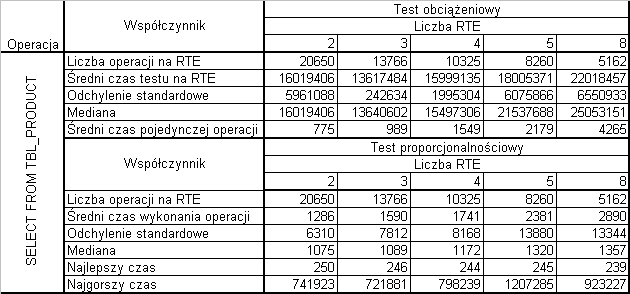
\includegraphics[width=0.9\linewidth]{figures/time_tab01.png}
\end{center}
\caption{Czasy wykonania operacji selekcji produktu}\label{tab:time_tab01}
\end{table}

\begin{table}[h]
\begin{center}
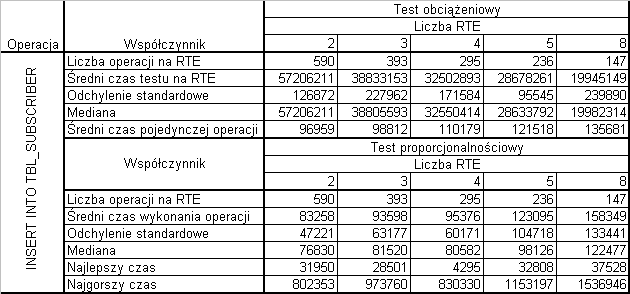
\includegraphics[width=0.9\linewidth]{figures/time_tab02.png}
\end{center}
\caption{Czasy wykonania operacji wstawienia osoby do listy subskrybcji}\label{tab:time_tab02}
\end{table}

\begin{table}[h]
\begin{center}
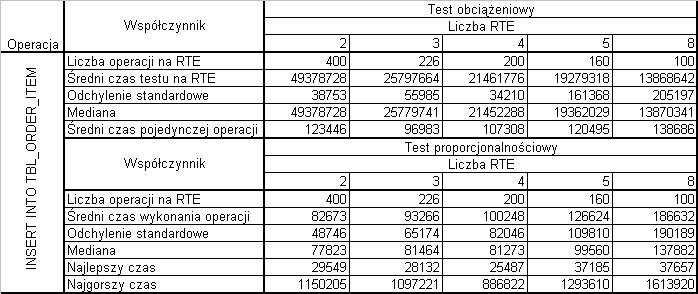
\includegraphics[width=0.9\linewidth]{figures/time_tab03.png}
\end{center}
\caption{Czasy wykonania operacji dodania produktu do zamówienia}\label{tab:time_tab03}
\end{table}

\begin{table}[h]
\begin{center}
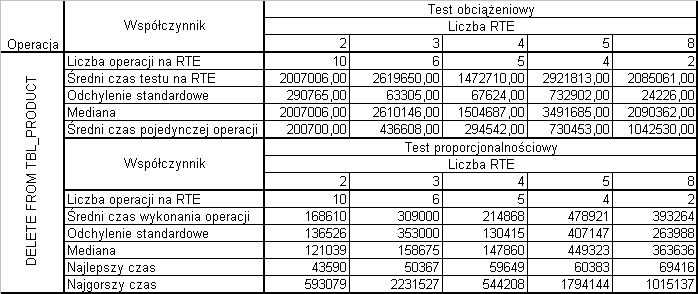
\includegraphics[width=0.9\linewidth]{figures/time_tab04.png}
\end{center}
\caption{Czasy wykonania operacji usunięcia produktu}\label{tab:time_tab04}
\end{table}

 
\chapter{Opis techniczny benchmarku}
\section{Streszczenie}
Załącznik ten jest przeznaczony dla osób, które w przyszłości chciałyby rozszerzać,
rozbudowywać omawiany system np.: studentów kolejnych roczników. Jego celem jest zatem dostarczenie
możliwie jak największej porcji użytecznych informacji dla takich osób.

Omawiany w tej pracy benchmark powstawał na zasadzie prototypowania i określania przyrostów funkcjonalnych,
gdyż nie można było już na samym początku prac, przewidzieć dokładnie 
jego architektury. Na taki stan rzeczy złożyło się kilka faktów:
\begin{itemize}
\item Autor benchmarku w momencie rozpoczynania prac nie posiadał doświadczenia związanego z budową tego typu
rozwiązań, w związku z czym nie był w stanie przewidzieć wszystkich problemów jakie na jego drodze mogły się
pojawić.
\item Budowane rozwiązanie nie posiadało innego adekwatnego pierwowzoru, na którym można było by się w pełni oprzeć.
Wspomniany w rozdziale \ref{chap:teo} benchmark TPC-C pod wieloma względami różnił się od planowanego systemu.
\end{itemize}
Przyjęcie tego typu strategii jest bardzo często stosowane podczas budowy rozwiązań eksperymentalnych, 
w których trudno jest przewidzieć do końca architekturę. Poza stworzeniem systemu, równorzędnym celem 
było zdobycie doświadczenia i wyciągnięcie wniosków odnośnie przyjętych założeń projektowych.

W przypadku pytań/uwag do niniejszej pracy autor oferuje swoją pomoc. W tym celu należy kontaktować się 
poprzez adres email: mirek.begier@gmail.com.

\section{Fizyczna struktura systemu}
Omawiane rozwiązanie zostało wykonane w oparciu o środowisko Eclipse w wersji 3.2.
System składa się z 4 projektów:
\begin{itemize}
\item JXmlSerializer -- jest to projekt biblioteki dostępu do plików xml poprzez stosowanie adnotacji klas.
Klasy takie są następnie serializowane i deserialiozwane do formatu xml. Idea tej biblioteki została zaczerpnięta
ze środowiska .Net~\cite{.Net1}~\cite{.NetXmlSerializer1}, w którym istnieje podobny mechanizm oparty o atrybuty. 
W stworzonym benchmarku biblioteka została wykorzystana w celu uproszczenia odczytywania i zapisywania plików xml reprezentujących:
\begin{itemize}
\item model bazy danych -- pakiet org.jdbmeasure.model.database,
\item model obciążenia bazy danych -- pakiet org.jdbmeasure.model.load,
\item model testu -- pakiet org.jdbmeasure.model.test,
\item plik konfiguracyjny klienta RTE -- pakiet org.jdbmeasure.rte.config.
\end{itemize}
Dla każdego z tych plików istnieją klasy z adnotacjami, stąd w powyższym wyliczeniu występują po myślniku nazwy pakietów,
zawierających te klasy. Bliższy opis biblioteki JXmlSerializer znajduje się dalej.%punkcie \ref{xmlser}.
\item JDBMeasure -- projekt ten zawiera klasy i pakiety stanowiące korzeń systemu. Bliższy opis znajduje się w dalszej części pracy.
\item JDBMeasureRCP -- projekt ten zawiera klasy i pakiety dotyczące interfejsu graficznego serwera benchmarku. Projekt ten
jest projektem aplikacji serwera, zgodnej z architekturą Eclipse RCP. Znajdują się tutaj zatem:
\begin{itemize}
\item widoki,
\item edytory,
\item okna dialogowe,
\item kreatory.
\end{itemize}
Projekt ten korzysta z klas zawartych w projekcie JDBMeasure, jego głównym zadaniem jest wizualizacja zawartych tam mechanizmów benchmarku.
\item JDBMeasureRCPExtJars -- jest projektem specyficznym dla aplikacji Eclipse RCP, zawiera on wszystkie biblioteki zewnętrzne dla tego typu aplikacji.
Znajdują się tutaj zatem wyłącznie pliki jar bibliotek takich jak:
\begin{itemize}
\item Hibernate 3.1~\cite{Hibernate1},
\item Hibernate Annotation 3.1~\cite{HibernateAnn1},
\item Spring 2.0~\cite{Spring1},
\item JFreeChart 1.0.1~\cite{JFreeChart1}.
\end{itemize} 
Umieszczenie plików jar w osobnym projekcie jest niezbędne ze względu na mechanizmy bezpieczeństwa i hierarchię ClassLoader'ów
aplikacji RCP.
\end{itemize}

\section{JXmlSerializer -- opis biblioteki}%\label{xmlser}
JXmlSerializer jest narzędziem do serializacji i deserializacji obiektów do formatu xml,
biblioteka ta powstała niezależnie od budowanego benchmarku, w celu ułatwienia pracy z dokumentami xml.
Główna klasa biblioteki używa adnotacji do tworzenia mapowań obiektów na dokumenty xml.
Poniżej zamieszczono przykładową klasę wraz z mapowaniami jej pól do dokumentu xml. 
\begin{quote}
\begin{Verbatim}
@XmlRoot("person")
public class Person {
	private String firstname;
	private String surname;
	private String description;
	private Sex sex;

	@XmlAttribute("firstname")
	public String getFirstname() {
		return this.firstname;
	}
	public void setFirstname(String firstname) {
		this.firstname = firstname;
	}

	@XmlAttribute("surname")
	public String getSurname() {
		return this.surname;
	}
	public void setSurname(String surname) {
		this.surname = surname;
	}

	@XmlElement("description")
	public String getDescription() {
		return description;
	}
	public void setDescription(String description) {
		this.description = description;
	}
	
	@XmlAttribute("sex")
	public Sex getSex() {
		return sex;
	}
	public void setSex(Sex sex) {
		this.sex = sex;
	}
}
\end{Verbatim}
\end{quote}
A zatem jedyne co należy zrobić by móc używać tej biblioteki, jest użycie we własnej klasie adnotacji 
z pakietu org.jxmlserializer.annotations, a następnie można już bardzo łatwo serializować obiekty:
\begin{quote}
\begin{Verbatim}
JXmlSerializer<Person> serializer 
	= new JXmlSerializer<Person>(Person.class);
serializer.serialize(file, person);
\end{Verbatim}
\end{quote}
oraz je deserializować z dokumentów xml:
\begin{quote}
\begin{Verbatim}
JXmlSerializer<Person> serializer 
	= new JXmlSerializer<Person>(Person.class);
Person person = serializer.deserialize(file);
\end{Verbatim}
\end{quote}
Powyższe informacje są wystarczające do zrozumienia kontekstu zastosowania biblioteki w omawianym benchmarku.
Głównym powodem wydzielenia kodu tej biblioteki, jako oddzielnego projektu, była jej uniwersalność -- biblioteka ta
może znaleźć zastosowanie wszędzie tam, gdzie pracuje się z dokumentami xml.

\section{JDBMeasure - omówienie projektu}
Jak już wspomniano JDBMeasure jest głównym projektem benchmarku, skupia on bowiem wszystkie te klasy,
które wykonują kod związany z główną funkcjonalnością aplikacji. Struktura tego projektu składa się 
z następujących katalogów:
\begin{quote}
\begin{Verbatim}
<DIR>          bin -- katalog skompilowanych klas,
   5 538 build.xml -- plik projektu anta,
<DIR>          doc -- katalog zawierający dokumentację, 
<DIR>          etc -- szablony i  dodatki,
<DIR>          ftp -- kod źródłowy serwera ftp,
<DIR>          lib -- wymagane biblioteki,
<DIR>          src -- kody źródłowe klas,
<DIR>          test -- kody źródłowe testów jednostkowych.
\end{Verbatim}
\end{quote}
Katalog doc zawiera ogólnie rozumianą dokumentację:
\begin{itemize}
\item JavaDoc kodu źródłowego -- podkatalog /doc/javadoc,
\item prezentacje benchmarku przygotowywane w ramach seminarium dyplomowego -- podkatalog /doc/presentations,
\item opis XmlSchema dla modeli -- podkatalog /doc/xmlschemas,
\item notatki -- podkatalog /doc/notes,
\item oraz pracę magisterską w LaTex'u -- podkatalog /doc/mgr/desc.
\end{itemize}
Nie mniej jednak najważniejsze w tym projekcie są kody źródłowe klas z katalogu src. 
Struktura pakietów przedstawia się następująco:
\begin{quote}
\begin{Verbatim}
\---org
    \---jdbmeasure
        +---database
        |   \---generator
        |       \---column
        |           \---exception
        +---model
        |   +---database
        |   |   \---classbuilder
        |   +---load
        |   \---test
        +---rte
        |   +---config
        |   +---info
        |   \---test
        |       \---properties
        +---server
        |   +---config
        |   \---info
        +---test
        |   +---datasource
        |   +---result
        |   \---script
        |       +---generator
        |       \---metadata
        \---util
            +---beans
            +---file
            +---math
            \---net\end{Verbatim}
\end{quote}
W dalszej części tego punktu zostaną omówione poszczególne pakiety
\subsection{Pakiet org.jdbmeasure.database}
Pakiet org.jdbmeasure.database zawiera klasy wykorzystywane podczas tworzenia populacji bazy danych,
jak i skryptów testowych. Większość klas tego pakietu służy do generowania danych poszczególnych kolumn, rekordów czy relacji.
Na rys.~\ref{rys:uml01} przedstawiono uproszczony diagram klas tego pakietu.
\begin{figure}[h]
\begin{center}
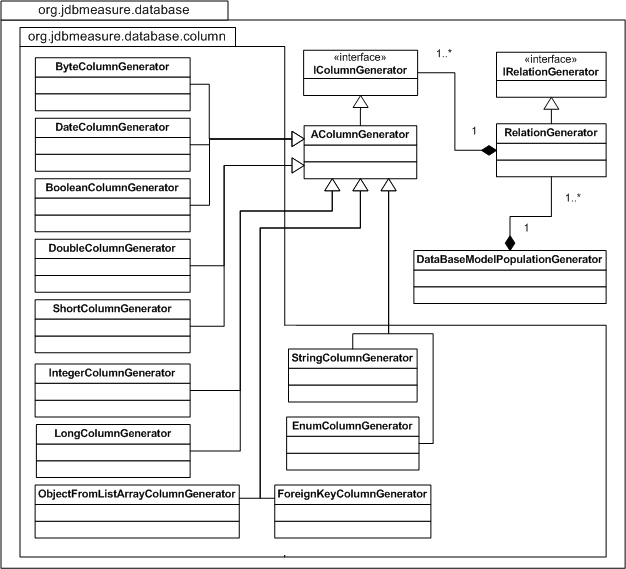
\includegraphics[width=1.0\linewidth]{figures/uml01.png}%[width=0.9\linewidth]
\end{center}
\caption{Diagram klas pakietu org.jdbmeasure.database}\label{rys:uml01}
\end{figure}
Klasa DataBaseModelPopulationGenerator jest odpowiedzialna za tworzenie populacji bazy danych. Znaczną część tego pakietu
stanowią klasy implementujące interfejs IColumnGenerator, są to klasy generatorów kolumn różnego typu wartości. 

\subsection{Pakiet org.jdbmeasure.model}
Pakiet ten zawiera klasy reprezentujące trzy modele opisujące razem test.
Klasy te zawierają adnotacje umożliwiające ich serializację z wykorzystaniem biblioteki JXmlSerializer,
do dokumentów xml. Dla każdego z trzech modeli wyodrębniono oddzielny podpakiet:
\begin{itemize}
\item org.jdbmeasure.model.database -- dla modelu bazy danych,
\begin{figure}[h]
\begin{center}
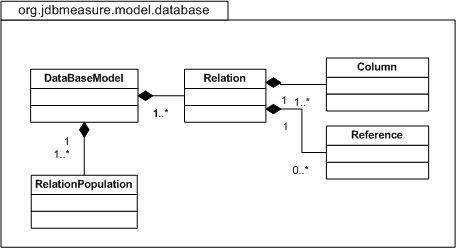
\includegraphics[width=0.8\linewidth]{figures/uml02.png}
\end{center}
\caption{Diagram klas pakietu org.jdbmeasure.model.database}\label{rys:uml02}
\end{figure}
\item org.jdbmeasure.model.load -- dla modelu obciążenia,
\begin{figure}[h]
\begin{center}
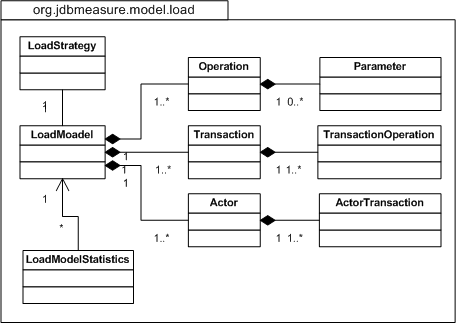
\includegraphics[width=0.8\linewidth]{figures/uml03.png}
\end{center}
\caption{Diagram klas pakietu org.jdbmeasure.model.load}\label{rys:uml03}
\end{figure}
\item org.jdbmeasure.model.test -- dla modelu testu.

\begin{figure}[h]
\begin{center}
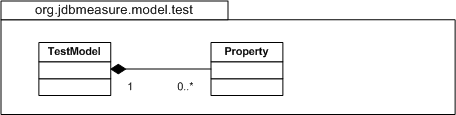
\includegraphics[width=0.8\linewidth]{figures/uml04.png}
\end{center}
\caption{Diagram klas pakietu org.jdbmeasure.model.test}\label{rys:uml04}
\end{figure}

\end{itemize} 

\subsection{Pakiet org.jdbmeasure.rte}
Pakiet org.jdbmeasure.rte zawiera główne klasy klienta RTE. Najważniejsze z nich to:
\begin{itemize}
\item RteClient -- klasa ta implementuje interfejs IRteClient. Jest to interfejs udostępniany poprzez RMI serwerowi benchmarku.
Interfejs IRteClient służy do komunikacji pomiędzy serwerem, a klientem RTE. W związku z tym klasa RteClient jest klasą implementującą
interfejs komunikacyjny z serwerem.
\item ScriptExecutor -- klasa ta służy do wykonywania skryptów testowych.
\item SignalMonitor -- jest to klasa służąca do przekazywania sygnałów synchronizujących pomiędzy klientem RTE a serwerem.
\item RteBeanInfo -- klasa ta dostarcza informacji o środowisku uruchomieniowym klienta RTE. Informacje te dotyczą głównie
ścieżek do katalogów bibliotek, plików wejściowych i wyjściowych, a także sterownika JDBC.
\end{itemize}
Na~rys.~\ref{rys:uml05} przedstawiono diagram klas pakietu org.jdbmeasure.rte.
\begin{figure}[h]
\begin{center}
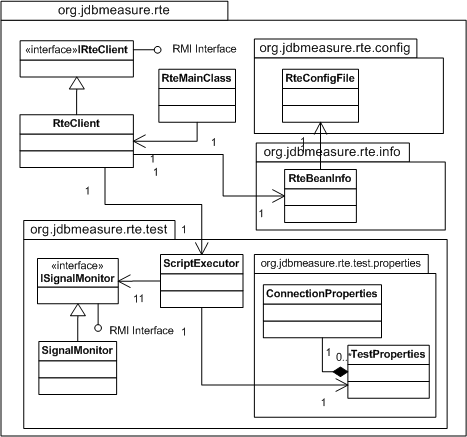
\includegraphics[width=0.8\linewidth]{figures/uml05.png}
\end{center}
\caption{Diagram klas pakietu org.jdbmeasure.rte}\label{rys:uml05}
\end{figure}

\subsection{Pakiet org.jdbmeasure.server}
Pakiet ten zawiera główne klasy serwera benchmarku, a także klasę aplikacji konsolowej (ServerMainClass).
Na~rys.~\ref{rys:uml06} przedstawiono diagram klas tego pakietu. Na uwagę zasługuje interfejs IBenchmarkServer,
jest to interfejs udostępniany klientom RTE poprzez protokół RMI . Klienci wykorzystują go w procesie komunikacji
z serwerem benchmarku. Klasa BenchmarkServer jest implementacją tego interfejsu. Dostarcza ona mechanizmy komunikacji
klient--serwer na wszystkich jej etapach począwszy od połączenia i rejestracji, poprzez deploye'owanie testów,
a skończywszy na przeprowadzaniu procedury testowej i zbieraniu wyników pomiarów.
\begin{figure}[h]
\begin{center}
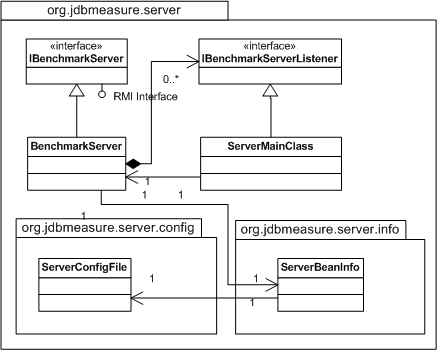
\includegraphics[width=0.8\linewidth]{figures/uml06.png}
\end{center}
\caption{Diagram klas pakietu org.jdbmeasure.server}\label{rys:uml06}
\end{figure}

\subsection{Pakiet org.jdbmeasure.test}
Pakiet ten skupia klasy związane z tworzeniem skryptów testowych, oraz analizą wyników testów (zob.~rys.~\ref{rys:uml07}).
Główną klasą jest tutaj klasa Test, jest ona fasadą dla całego pakietu -- komunikacja z innymi klasami odbywa się bezpośrednio
przez nią. W pakiecie tym możemy wyróżnić trzy podpakiety:
\begin{itemize}
\item org.jdbmeasure.test.datasource -- pakiet klas źródła danych dla klienta RTE, podczas procedury testu.
\item org.jdbmeasure.test.testresult -- pakiet klas reprezentujących przeanalizowany rezultat testu.
\item org.jdbmeasure.test.script -- pakiet klas odpowiedzialnych za generowanie poszczególnych operacji i 
przechowywania metadanych skryptów testowych.
\end{itemize}
\begin{figure}[h]
\begin{center}
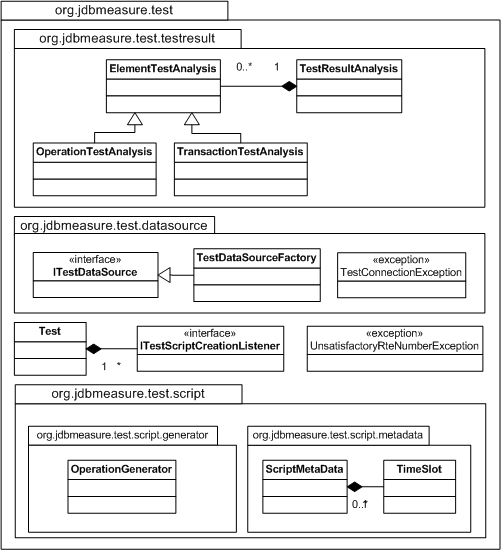
\includegraphics[width=0.8\linewidth]{figures/uml07.png}
\end{center}
\caption{Diagram klas pakietu org.jdbmeasure.test}\label{rys:uml07}
\end{figure}

\subsection{Pakiet org.jdbmeasure.util}
Na pakiet ten składa się grupa niepowiązanych klas, które można określić mianem klas pomocniczych. Do pakietu tego 
należą klasy takie jak:
\begin{itemize}
\item JarClassLoader -- klasa ułatwiająca ładowanie klas z wybranej biblioteki jar.
\item JavaCompiler -- klasa automatyzująca proces kompilacji klas ze wskazanych katalogów, z wykorzystaniem wskazanych bibliotek.
\item FileUtil -- klasa obudowująca podstawowe operacje na plikach i katalogach.
\item FreePortFinder -- klasa ułatwiająca znalezienie wolnego portu.
\item MathExp, MathUtil -- klasy ułatwiające korzystanie z typów BigInteger oraz BigDecimal, a także dostarczające szeregu użytecznych funkcji matematycznych.
\end{itemize}

W bieżącym punkcie zostały omówione główne pakiety projektu JDBMeasure, bliższe informacje 
odnośnie, każdej z klas można znaleźć w dokumentacji JavaDoc.

\section{JDBMeasureRCP - omówienie projektu}
Projekt JDBMeasureRCP jest projektem aplikacji graficznego serwera benchmarku. Jest to aplikacja 
zgodna z modelem Eclipse RCP. Poniżej zamieszczono strukturę pakietów tego projektu. 
\begin{quote}
\begin{Verbatim}
\---org
    \---jdbmeasure
        \---rcp
            +---action -- akcje
            +---bean -- klasy dostosowujące klasy z projektu JDBmeasure 
            +---dialog -- klasy okien dialogowych
            +---editor -- klasy edytorów
            |   +---common
            |   +---databasemodel -- klasy edytora modelu bazy danych
            |   |   +---dialog
            |   |   \---editorpart
            |   +---loadmodel -- klasy edytora modelu obciążenia
            |   |   +---dialog
            |   |   \---editorpart
            |   \---testmodel -- klasy edytora modelu testu
            |       \---editorpart
            +---view -- klasy widoków drzewa i listy podłączonych rte
            +---wizard -- klasy kreatora projektu testu
            \---xmleditor -- klasy edytora xml
\end{Verbatim}
\end{quote}
Projekt ten korzysta z bibliotek zawartych w projekcie JDBMeasureRCPExtJars, który został utworzony
eclipsowym kreatorem ,,Plugin from existing JAR archives''. Do stworzenia wersji gotowej do rozpowszechniania,
należy posłużyć się produktem JDBMeasure.product, wykonując dla niego polecenie ,,Eclipse product export wizard''.

\section{Podsumowanie}
Niniejszy rozdział stanowi opis techniczny benchmarku. Uzupełnieniem tego opisu może być dokumentacja JavaDoc,
dostępna w katalogu /doc/javadoc projektu JDBMeasure. Autor aplikacji dołożył wszelkich starań by w przyszłości
aplikacja była łatwa w rozwoju. W przypadku pytań/problemów służy również swoją pomocą.
 

\end{document}
